\documentclass[12pt]{article}
\usepackage[UTF8]{ctex}
\usepackage[textwidth=450bp,vmargin=2.5cm]{geometry}%设置页边距
\setlength{\parskip}{0.5em}
\usepackage{array} %主要是增加列样式选项
\usepackage[dvipsnames]{xcolor}%颜色宏包
\usepackage{graphicx}%图片宏包
\usepackage{subfigure}%并排图片.
\usepackage{wrapfig}
\usepackage{amsmath}%公式宏包
\usepackage{threeparttable}%表格注释
\usepackage[T1]{fontenc}    %字体编码
\usepackage{newtxtext, newtxmath}  %两种使用Times New Roman 字体的方法
\usepackage{subfigure}%并排图片
\usepackage{float}
\newcommand \dbar {{\; \bar{} \hspace{-0.3em} \mathrm d}}%设置dbar
\usepackage{hyperref}%超链接
\hypersetup{hypertex=true,
	colorlinks=true,
	linkcolor=blue,
	anchorcolor=blue,
	citecolor=blue}%超链接

\begin{document}
	热统
	\newpage
	\tableofcontents
	\section{数学基础}
	\par 对于$F(x,y,z)=0$,有$\mathrm{d}F=\frac{\partial F}{\partial x}\mathrm{d}x +\frac{\partial F}{\partial y}\mathrm{d}y + \frac{\partial F}{\partial z}\mathrm{d}z=0$
	\quad 有以下结论:
	\begin{equation}
		(\frac{\partial z}{\partial x})_y=1/(\frac{\partial x}{\partial z})_y
	\end{equation}
\begin{equation}
	(\frac{\partial y}{\partial x})_z (\frac{\partial x}{\partial z})_y (\frac{\partial z}{\partial y})_x =-1
   \label{x1}
\end{equation}
其中(\ref{x1})的证明如下:
 分别令$\mathrm{d}z,\mathrm{d}y,\mathrm{d}x=0$,可以得到
\begin{equation}
	\begin{split}
	(\frac{\partial y}{\partial x})_z&=-\frac{(\partial F/\partial x)_{y,z}}{(\partial F/\partial y)_{x,z}}\\
		(\frac{\partial x}{\partial z})_y&=-\frac{(\partial F/\partial z)_{x,y}}{(\partial F/\partial x)_{y,z}}\\
			(\frac{\partial z}{\partial y})_x&=-\frac{(\partial F/\partial y)_{x,z}}{(\partial F/\partial z)_{x,y}}\\
			\end{split}
\end{equation}
把3式相乘即可得证。
\par 雅可比行列式\\
定义:
\begin{equation}
	\frac{\partial(y_1,y_2,...,y_n)}{\partial(x_1,x_2,...,x_n)}=\left| \begin{matrix}
		\frac{\partial {{y}_{1}}}{\partial {{x}_{1}}} & \frac{\partial {{y}_{1}}}{\partial {{x}_{2}}} & ... & \frac{\partial {{y}_{1}}}{\partial {{x}_{n}}}  \\
		\frac{\partial {{y}_{2}}}{\partial {{x}_{1}}} & \frac{\partial {{y}_{2}}}{\partial {{x}_{2}}} & ... & \frac{\partial {{y}_{n}}}{\partial {{x}_{n}}}  \\
		... & ... & ... & ...  \\
		\frac{\partial {{y}_{n}}}{\partial {{x}_{1}}} & \frac{\partial {{y}_{n}}}{\partial {{x}_{2}}} & ... & \frac{\partial {{y}_{n}}}{\partial {{x}_{n}}}  \\
	\end{matrix} \right|
\end{equation}
其具有性质:
\begin{equation}
	(\frac{\partial y}{\partial x_1})_{x_2}=\frac{\partial (y,x_2)}{\partial(x_1,x_2)}
\end{equation}
证明上式只需要注意到$x_1,x_2$相互独立,因此$\partial x_2/\partial x_1=0$。此外还有以下性质:
\begin{equation}
	\begin{split}
	\frac{\partial (y_2 ,y_1,...,y_n)}{\partial (x_1,x_2,..,x_n)}&=-\frac{(y_1,y_2,...,y_n)}{(x_1,x_2,...,x_n)}\\ \quad \\
	\frac{\partial (y_1 ,y_2,...,y_n)}{\partial( x_1,x_2,..,x_n)}&=\frac{\partial (y_1 ,y_2,...,y_n)}{\partial (u_1,u_2,..,u_n)}\frac{\partial (u_1 ,u_2,...,u_n)}{\partial (x_1,x_2,..,x_n)}\\ \quad \\
	\frac{\partial (y_2 ,y_1,...,y_n)}{\partial (x_1,x_2,..,x_n)}&=1/\frac{\partial (x_1,x_2,..,x_n)}{\partial (y_1 ,y_2,...,y_n)}
	\end{split}
\end{equation}
\par 全微分条件
\\对于函数$z=z(x,y)$一般认为给出的函数性质足够好,有以下性质:
\begin{equation}
	\frac{{{\partial }^{2}}z}{\partial x\partial y}=\frac{{{\partial }^{2}}z}{\partial y\partial x}
	\label{x34}
\end{equation}

一个近似等式,当$n$是一个很大的数时,有:
\begin{equation}
	\ln n!=n(\ln n-1)
\end{equation}
证明:\\
当$n$很大时,$\ln n!$的导数为:
\begin{equation}
	\frac{\mathrm{d}\ln n!}{\mathrm{d}n}=\ln (n+1)!-\ln n!=\ln (n+1)\simeq \ln n
	\label{x53}
\end{equation}
同时有:
\begin{equation}
	\ln n!=\ln 1+\ln 2+...+\ln n=\sum_{1}^{n} \ln m
\end{equation}
当$n\to \infty$时:
\begin{equation}
	\ln n!=\int_{1}^{n}\ln x\mathrm{d}x=n\ln n-n+1\simeq n(\ln n-1)
\end{equation}
很容易检验上式并没有改变其导数(\ref{x53})。

积分因子:\\
如果微分式$\mathrm{d}z=X(x,y)\mathrm{d}x+Y(x,y)\mathrm{d}y$不满足全微分条件(\ref{x34}),但存在$\lambda$使得:
\begin{equation}
	\lambda \mathrm{d}z=\lambda X\mathrm{d}x+\lambda Y\mathrm{d}y
\end{equation}
满足全微分条件:
\begin{equation}
	\frac{\partial}{\partial x}\lambda Y=\frac{\partial }{\partial y} \lambda X
\end{equation}
那么可以令$\mathrm{d}s=\lambda\mathrm{d}z$,即$\lambda \mathrm{d}z$是一个全微分,对于$\psi(s)$是$s$的任意函数,有:
\begin{equation}
	\lambda \psi (s)\mathrm{d}z=\psi(s)\mathrm{d}s=\mathrm{d}\Psi
\end{equation}
其中$\Psi=\int \psi(s)\mathrm{d}s$,这表明$\lambda \psi(s)$也是$\mathrm{d}z$的积分因子。说明当一个微分式有一个积分因子时,它就有无穷多个积分因子,任意两个积分因子之比是$s$的函数。

连续性方程(这里用电荷守恒举例):
\begin{equation}
	\nabla \cdot \mathbf{J}+\frac{\partial \rho}{\partial t}=0
	\label{x35}
\end{equation}
其中$\mathbf{J}$是电流密度(通过某个截面的电流量),$\rho$是电荷密度对时间的变化率。\\
我们可以根据电荷守恒证明:
\begin{equation}
	I+\frac{\mathrm{d}\rho}{\mathrm{d} t}=0
\end{equation}
上式可写为:
\begin{equation}
	\oint \mathbf{J}\cdot \mathrm{d}\mathbf{S}+\frac{\mathrm{d}}{\mathrm{d}t}\int_{V}\rho \mathrm{d}V=0
\end{equation}
对第一项使用散度定理,第二项微分和积分交换次序:
\begin{equation}
	\int_V \nabla\cdot \mathbf{J}\mathrm{d}V+\int_V\frac{\partial}{\partial t}\rho\mathrm{d}V=0
\end{equation}
即:
\begin{equation}
	\int_V (\nabla \cdot \mathbf{J}+\frac{\partial }{\partial t}\rho)\mathrm{d}V=0
\end{equation}
这样就得到了连续性方程$\nabla \cdot \mathbf{J}+\frac{\partial \rho}{\partial t}=0$.

几个积分公式:\\
1.$I=\int_{-\infty}^{\infty}\mathrm{e}^{-x^2}\mathrm{d}x$:
\begin{equation}
	\begin{split}
	I^2&=\iint_{-\infty}^{\infty}\mathrm{e}^{-x^2-y^2}\mathrm{d}x\mathrm{d}y \\
	&=\int_{0}^{2\pi}\mathrm{d}\theta\int_{0}^{\infty}\mathrm{e}^{-r^2}r\mathrm{d}r\\
	&=\pi
\end{split}
\end{equation}
所以有:
\begin{equation}
	I=\sqrt{\pi}
\end{equation}
2.$\Gamma(n)=\int_{0}^{\infty}\mathrm{e}^{-x}x^{n-1}\mathrm{d}x$,其中$n$为整数或半整数:
\begin{equation}
	\Gamma(n)=(n-1)\Gamma(n-1)
\end{equation}
由:
\begin{equation}
	\left\{\begin{split}
&\Gamma(1)=\int_{0}^{\infty}\mathrm{e}^{-x}\mathrm{d}x=1\\
&\Gamma(\frac{1}{2})=\int_{0}^{\infty}\mathrm{e}^{-x}x^{-1/2}\mathrm{d}x=2\int_{0}^{\infty}	\mathrm{e}^{-y^2}\mathrm{d}y=I=\sqrt{\pi}
\end{split}\right.
\end{equation}
可知:
\begin{equation}
	\left\{\begin{split}
		\Gamma(n)&=(n-1)!\quad (n=1,2,3,...)\\
		\Gamma(n+\frac{1}{2})&=(n-\frac{1}{2})(n-\frac{3}{2})\cdot\cdot\cdot\frac{1}{2}\cdot\sqrt{\pi}\quad
	\end{split}
	\right.
\end{equation}



\newpage
\section{名词解释}
\noindent
孤立系:与外界没有物质交换,也没有能量交换的系统。

\noindent
闭系:与外界没有物质交换,但是有能量交换的系统。

\noindent
开系:与外界既有物质交换,也有能量交换的系统。

\noindent
热力学平衡态:孤立系统的各种宏观性质在长时间不发生任何改变。(其中的宏观性质可以用几何参量、力学参量、电磁参量和化学参量描述)

\noindent
弛豫时间:系统由初始状态到达平衡状态所经历的时间。

\noindent
广延量:与系统的质量或物质的量成正比。

\noindent
强度量:与系统的质量或物质的量无关。

\noindent
温度:表示物体冷热程度的物理量,微观上指的是物体分子热运动的剧烈程度。

\noindent
内能:系统中粒子无规则运动的总能量平均值。

\noindent
热力学第零定律:\\物体A和物体B各自与处在同一状态的物体C达到热平衡,则A与B进行热接触也将处于热平衡。

\noindent
热力学第一定律:\\自然界的一切物质都具有能量,能量有各种不同的形式,可以从一种形式转化成另一种形式,从一个物体传递到另一个物体,在传递和转化中能量的数量不变。(另一种表述:第一类永动机是不可能造成的。)

\noindent
热力学第二定律:\\
克劳修斯表述:不可能把热量从低温物体传到高温物体而不引起其他变化。\\
开尔文表述:不可能从单一热源吸热使之完全变成有用功而不引起其他的变化。\\
开尔文表诉:第二类永动机是不可能造成的。\\
熵增加原理:孤立系统的熵永不自动减少,熵在可逆过程中不变,在不可逆过程中增加。

\noindent
热力学第三定律:\\
1.能斯特定理:凝聚系的熵在等温过程中的改变随热力学温度趋于0。($ \underset{T\to 0}{\mathop{\lim }}\,{{(\Delta S)}_{T}}=0$)\\
2.绝对零度不能达到原理不可能通过有限步骤使一个物体冷却到热力学温度零度。\\
3.$\underset{T\to 0}{\mathrm{lim}}S_0=0$:$T\to 0K$时,同一物质处在热力学平衡的一切形态具有相同的熵。

\noindent
焦耳定律:气体的内能只能是温度的函数。

\noindent
阿伏伽德罗定律:在压强和温度相同的情况下,若气体体积相等则物质的量也相等。

\noindent
玻意耳定律:理想气体在物质的量(质量)不变的情况下压强$p$和体积$V$的乘积是一个定值($pV=Const$)。

\noindent
准静态过程:系统在经过一系列非常缓慢的过程,其中每一个状态都可以看作是一个平衡态,是一个理想的极限概念。  

\noindent
可逆过程:如果一个过程发生后,它所产生的影响可以完全消除而令一切恢复原状,那么该过程称为可逆过程。(推论:所有工作于两个确定温度之间的可逆热机效率相等。)

\noindent
卡诺定理:所有工作于两个确定的温度之间的热机中,可逆热机的效率最高。

\noindent
节流过程:多孔塞两边分别维持较高压强$p_1$和较低压强$p_2$,气体从高压一边不断流到低压一边并且达到定常态。(这个过程绝热等焓)

\noindent
焦汤效应(焦耳-汤姆孙效应):节流过程前后气体温度发生变化。(理想气体汤焦系数$\mu=(\frac{\partial T}{\partial p})_H=0$,节流过程温度不变。)

\noindent
绝热膨胀:准静态绝热过程中理想气体熵保持不变。

\noindent
热辐射:物体具有温度而辐射电磁波的现象。

\noindent
热传导:物质中大量的分子热运动相互撞击使能量从高温物体传给低温物体的过程。(严格来说只有固体才能发生,液体和气体热传导和热对流同时发生)

\noindent
热对流:液体或气体中较热部分和较冷部分通过循环流动使温度趋于均匀的过程。

\noindent
平衡辐射:辐射体对电磁波的吸收和辐射达到平衡,热辐射的特性将只取决于温度,与辐射体的其它特性无关,称为平衡辐射。

\noindent
相:在没有外力作用下,物理、化学性质完全相同、成分相同的均匀物质的聚集态。

\noindent
单元系:化学上纯的物质,只含一种化学成分(一个组元)。

\noindent
多元系:含有两种或两种以上的化学组成的系统。

\noindent
饱和蒸气:与凝聚相(液体或固体)达到平衡的蒸气。

\noindent
亨利定律:理想溶液中某溶质的蒸气分压与该溶质中的摩尔分数成正比($p_i\propto x_i$)。

\noindent
全同粒子系统:由具有完全相同的内禀属性(质量、电荷、自旋等)的同类粒子组成的系统。

\noindent
玻色子:自旋量子数为整数的微观粒子。(不遵守Pauli不相容原理)

\noindent
费米子:自旋量子数为半整数的微观粒子。(遵守Pauli不相容原理)

\noindent
等概率原理:对于处在平衡态的孤立系统,系统各个可能的微观状态出现的概率是相等的。

\noindent
能量均分定律:对于处在温度为$T$的平衡状态的经典系统,粒子能量中每一个独立的平方项的平均值等于$\frac{1}{2}kT$







\newpage
\section{热力学}
\subsection{热力学基本规律}
\subsubsection{与物态方程有关的几个系数}
\noindent
体胀系数$\alpha$:
\begin{equation}
	\alpha=\frac{1}{V}(\frac{\partial V}{\partial T})_p
\end{equation}	
压强系数$\beta$:
\begin{equation}
	\beta=\frac{1}{p}(\frac{\partial p}{\partial T})_V
\end{equation}	
等温压缩系数$\kappa_T$:
\begin{equation}
	\kappa_T=-\frac{1}{V}(\frac{\partial V}{\partial p})_T
\end{equation}	
\subsubsection{物态方程}
\noindent
温度与状态参量之间满足的方程:
\begin{equation}
	f(x_1,x_2,...x_n,T)=0
\end{equation}
其中$x_1,x_2,...,x_n$代表不同的状态参量。\\
 理想气体:
\begin{equation}
	PV=nRT
\end{equation}
范德瓦尔斯方程:
\begin{equation}
	(p+\frac{an^2}{V^2})(V-nb)=nRT
\end{equation}
顺磁性物质(居里定律,在(\ref{x45})中证明):
\begin{equation}
	\mathscr{M}=\frac{C}{T} \mathscr{H}
	\label{x44}
\end{equation}
其中$\mathscr{M}$是单位体积的磁矩(磁化强度),$\mathscr{H}$是磁场强度,$C$是待定常数。\\
对于简单液体和固体,有:
\begin{equation}
	V(T,p)=V_0(T_0,0)[1+\alpha (T-T_0)-\kappa_T p]
\end{equation}
证明如下:\\
以$p,V$为状态参量的物态方程可以把体积$V$写成温度$T$和压强$p$的函数:
\begin{equation}
	V=V(T,p)
\end{equation}
那么其全微分:
\begin{equation}
	\mathrm{d}V=(\frac{\partial V}{\partial T})_p\mathrm{d}T+(\frac{\partial V}{\partial p})_T\mathrm{d}p
\end{equation}
根据前面体胀系数$\alpha$和等温压缩系数$\kappa_T$的定义式很容易看出:
\begin{equation}
\begin{split}	
\frac{\mathrm{d}V}{V}&=\frac{1}{V}(\frac{\partial V}{\partial T})_p\mathrm{d}p+\frac{1}{V}(\frac{\partial V}{\partial p})_T\mathrm{d}T \\
&=\alpha \mathrm{d}T-\kappa_T \mathrm{d}p
\end{split}
\end{equation}
两边同时积分得:
\begin{equation}
	\ln V=\int{\alpha \text{d}T-{{\kappa }_{T}}\text{d}p}
\end{equation}
若$P$和$T$都分别随 $\alpha$和$\kappa_T$线性变化,则:
\begin{equation}
	\frac{V}{V_0}=\mathrm{e}^{\alpha (T-T_0)- \kappa_Tp}
\end{equation}
其中取$p_0=0$。\\
对于简单液体和固体它们的$\alpha$和$\kappa_T$都很小,那么将指数展开到一阶小量,即可得:
\begin{equation}
	V(T,p)=V_0(T_0,0)[1+\alpha (T-T_0)-\kappa_T p]
\end{equation}
\subsubsection{热容和焓}
\noindent
等容热容:
\begin{equation}
	C_V=\underset{\Delta T\to 0}{\mathop{\lim }}(\frac{\Delta Q}{T})_V=(\frac{\partial U}{\partial T})_V
\end{equation}
等压热容:
\begin{equation}
	C_p=\underset{\Delta T\to 0}{\mathop{\lim}}(\frac{\Delta Q}{T})_p=(\frac{\partial U+p\Delta V}{\partial T})_p=(\frac{\partial U}{\partial T})_p+p(\frac{\partial V}{\partial T})_p
\end{equation}
引入状态函数焓$H$,焓变表示等压过程中吸收的热量:
\begin{equation}
\begin{split}
	H&=U+pV	
\\	C_p&=(\frac{\partial H}{\partial T})_p	
\end{split}
\end{equation}
\subsubsection{理想气体绝热过程}
\noindent
对于理想气体的热容:
\begin{equation}
	C_V=\frac{\mathrm{d}U}{\mathrm{d}T}\quad \quad \quad C_p=\frac{\mathrm{d}H}{\mathrm{d}T}
\end{equation}
理想气体的焓:
\begin{equation}
	H=U+PV=U+nRT
\end{equation}
因此可得$C_V$与$C_p$的关系:
\begin{equation}
	C_p=C_V+nR
\end{equation}
定义比热容比$\gamma=C_p/C_V$,那么$C_V$和$C_p$的用$\gamma$表示为:
\begin{equation}
	C_V=\frac{nR}{\gamma-1}\quad \quad \quad C_p=\gamma \frac{nR}{\gamma-1}
\end{equation}
对于绝热过程,我们从$\mathrm{d}U=\mathrm{d}Q+\mathrm{d}W$中$\mathrm{d}Q=0$,可以得到(注意是理想气体):
\begin{equation}
	C_V\mathrm{d}T+p\mathrm{d}V=0
	\label{x2}
\end{equation}
把理想气体写出微分形式:
\begin{equation}
	p\mathrm{d}V+V\mathrm{d}P=nR\mathrm{d}T=C_V(\gamma-1)\mathrm{d}T
\end{equation}
根据(\ref{x2})把$C_V\mathrm{d}T$换成$-p\mathrm{d}V$可得微分方程:
\begin{equation}
	V\mathrm{d}p+\gamma p\mathrm{d}V=0
\end{equation}
显然可以得到理想气体绝热关系:
\begin{equation}
	pV^\gamma=Const
\end{equation}
根据理想气体状态方程的简单代换,可以得到:
\begin{equation}
	TV^{\gamma-1}=Const \quad \quad \quad \frac{T^\gamma}{p^{\gamma-1}}=Const
\end{equation}
\begin{wrapfigure}[3]{r}{8em}
	\begin{center}
		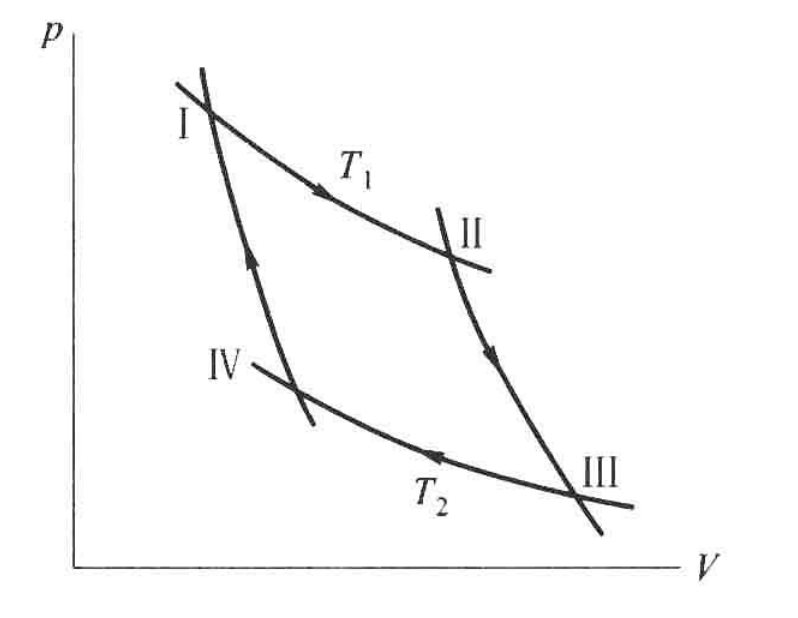
\includegraphics[width=1.5in]{F1.png}
		\label{F1}
	\end{center}
\end{wrapfigure}
\subsubsection{理想气体卡诺循环}
\noindent

卡诺循环包括4个过程,图(\ref{F1})中\uppercase\expandafter{\romannumeral1}到\uppercase\expandafter{\romannumeral2}和\uppercase\expandafter{\romannumeral3}到\uppercase\expandafter{\romannumeral4}为等温过程,\uppercase\expandafter{\romannumeral2}到\uppercase\expandafter{\romannumeral3}和\uppercase\expandafter{\romannumeral4}到\uppercase\expandafter{\romannumeral1}为绝热过程。

\noindent \uppercase\expandafter{\romannumeral1}到\uppercase\expandafter{\romannumeral2}(等温过程):
\begin{equation}
	\left \{
	\begin{split}
		&W_1=-\int_{{{V}_{1}}}^{{{V}_{2}}}{pdV=-\int_{{{V}_{1}}}^{{{V}_{2}}}{\frac{nRT}{V}}}dV=-nR\ln \frac{{{V}_{2}}}{{{V}_{1}}}\\
		&Q_1=-W_1=nRT_1\ln \frac{V_2}{V_1}\\
	   &\Delta U_1=0
	\end{split}
\right.
\end{equation}
\uppercase\expandafter{\romannumeral2}到\uppercase\expandafter{\romannumeral3}(绝热过程,利用$PV^\gamma=C$)
\begin{equation}
	\left \{
	\begin{split}
		&W_2=-\int_{{{V}_{2}}}^{{{V}_{3}}}{pdV=-\int_{{{V}_{2}}}^{{{V}_{3}}}{\frac{C}{V^\gamma}}}dV=\frac{C}{\gamma-1}(\frac{1}{V_3^{\gamma-1}}-\frac{1}{V_2^{\gamma-1}}) \\
		&Q_2=0\\
		&\Delta U_2=W_2=\frac{C}{\gamma-1}(\frac{1}{V_3^{\gamma-1}}-\frac{1}{V_2^{\gamma-1}})
	\end{split}\right.
\end{equation}
\uppercase\expandafter{\romannumeral3}到\uppercase\expandafter{\romannumeral4}与\uppercase\expandafter{\romannumeral1}到\uppercase\expandafter{\romannumeral2}类似:
\begin{equation}
	\left \{
	\begin{split}
		&W_3=-nR\ln \frac{{{V}_{4}}}{{{V}_{3}}}\\
		&Q_3=-W_3=nRT_2\ln \frac{V_4}{V_3}\\
		&\Delta U_3=0
	\end{split}\right.
\end{equation}
\uppercase\expandafter{\romannumeral4}到\uppercase\expandafter{\romannumeral1}与\uppercase\expandafter{\romannumeral2}到\uppercase\expandafter{\romannumeral3}类似:
\begin{equation}
	\left \{
	\begin{split}
		&W_4=\frac{C}{\gamma-1}(\frac{1}{V_1^{\gamma-1}}-\frac{1}{V_4^{\gamma-1}}) \\
		&Q_4=0\\
		&\Delta U_4=W_4=\frac{C}{\gamma-1}(\frac{1}{V_1^{\gamma-1}}-\frac{1}{V_4^{\gamma-1}})
	\end{split}\right.
\end{equation}
\par
由于经历了卡诺循环后初始状态和末态温度相同,因此内能不发生变化,所以整个系统在循环过程中对外做功与吸收的净热量相同,同时吸收热源的热量就是\uppercase\expandafter{\romannumeral1}到\uppercase\expandafter{\romannumeral2}中计算出的$Q_1$,因此可以计算出卡诺热机效率:
\begin{equation}
	\eta=1-\frac{T_2}{T_1}
\end{equation}
计算过程:
\begin{equation}
	\begin{split}
	\eta=\frac{Q_1+Q_3}{Q_1}=\frac{T_1\ln \frac{V_2}{V_1}+T_2\ln \frac{V_4}{V_3}}{T_1\ln \frac{V_2}{V_1}}\\
	\label{x3}
\end{split}
\end{equation}
其中由于\uppercase\expandafter{\romannumeral2}到\uppercase\expandafter{\romannumeral3}和\uppercase\expandafter{\romannumeral4}到\uppercase\expandafter{\romannumeral1}为绝热过程,因此有:
\begin{equation}
	\begin{split}
		T_1V_2^\gamma&=T_2V_3^\gamma \\ T_1V_1^\gamma&=T_2V_4^\gamma
	\end{split}
\end{equation}
2式相除可以得到$V_2/V_1=V_3/V_4$,代入到(\ref{x3})中,可以得到:
\begin{equation}
	\eta=\frac{(T_1-T_2)\ln (V_2/V_1)}{T_1 \ln(V_2/V_1)}=1-\frac{T_2}{T_1}
\end{equation}
\subsubsection{关于热力学第二定律的几个证明}
\noindent
1.证明克劳修斯表诉与开尔文表述是等价的。\\
证明:

我们先证明充分性,考虑一个卡诺循环,工作物质从温度为$T_1$,的高温热源吸取热量$Q_1$,在温度为$T_2$的低温热源放出热量$Q_2$,对外作功$W=Q_1-Q_2$,如果克氏表述不成立,可以将热量$Q_2$从温度为$T_1$的低温热源送到温度为$T_2$的高温热源而不引起其它变化,则全部过程的最终后果是从温度为$T_1$的热源吸取$Q_1-Q_2$的热量,将之完全变成有用的功,这样开氏表述也就不能成立.

反之,我们再证明,如果开氏表述不成立,则克氏表述也不能成立.如果开氏表述不成立,一个热机能够从温度为$T_1$的热源吸取热量$Q_1$,使之全部转化为有用的功$W=Q_1$,就可以利用这个功来带动一个逆卡诺循环(从低温热源吸取热量$Q_2$,在高温热源放出热量$Q_1+Q_2$),整个过程的最终后果是将热量$Q_2$从温度为$T_2$的低温热源传到温度为$T_1$的高温热源而未引起其它变化,这样克氏表述也就不能成立。
\begin{figure}[h]
		\centering
	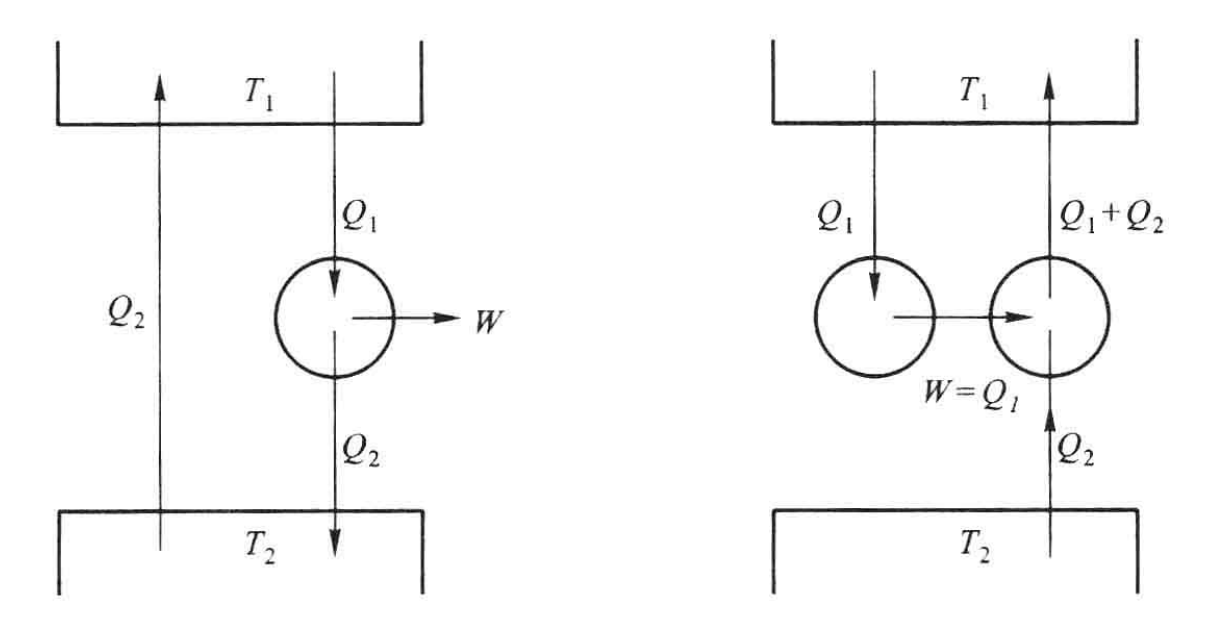
\includegraphics[scale=0.2]{F2.png}
\end{figure}
\\
\noindent
2.证明2条绝热线不能相交。\\
证明:

\begin{wrapfigure}[8]{r}{10em}
	\begin{center}
		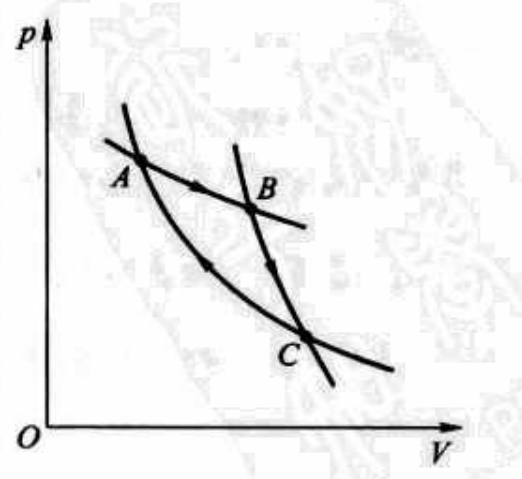
\includegraphics[width=2in]{F3.png}
		\label{F3}
	\end{center}
\end{wrapfigure}
假设在p-V图中两条绝热线交于C点,如图所示.设想一等温线与两条绝热线分别交于A点和B点(因为等温线的斜率小于绝热线的斜率,这样的等温线总是存在的),则在循环过程ABCA中,系统在等温过程AB中从外界吸取热量$Q$,而在循环过程中对外做功$W$,其数值等于三条线所围面积(正值)循环过程完成后,系统回到原来的状态,根据热力学第一定律,有$W=Q$,这样一来,系统在上述循环过程中就从单一热源吸热并将之完全转化为功了,这违背了热力学第二定律的开尔文表述,因此两条绝热线不可能相交。
\\

\noindent
3.证明卡诺定理。\\
\textcircled{1}反证法:

 设有可逆热机A效率为$\eta_A=\frac{W_1}{Q_1}$,不可逆热机B效率为$\eta_B=\frac{W_2}{Q_1 '}$,高温热源$T_1$,低温热源$T_2$,假设$\eta_A \leq \eta_B$,那么利用反证法证明假设不成立即可。\\
不妨设$Q_1=Q_1 '$,那么有$W_1\leq W_2$,则可以B从高温热源吸热$Q_1 '$,在低温热源放热$Q_2 '$,并利用$W_1$的功使A做逆循环(从低温热源吸热$Q_2$,在高温热源放热$Q_1$),剩余$W_2-W_1$用于对外做功,根据热力学第一定律,这一部分功必等于低温热源吸放热的差值:
\begin{equation}
	W_2-W_1=Q_2-Q_2'
\end{equation}
那么把A,B和热源看作一个整体可以得到一个系统使得从单一热源(低温热源)吸热使之完全变成功而不产生其他变化,与热力学第二定律相悖,故假设不成立,卡诺定理得证。

\noindent
\textcircled{2}用克劳修斯不等式证明

对于热机循环与多个热源交换热量,热机吸热的热源最高温度为$T_1$,热机放热的热源最低温度为$T_2$,根据克劳修斯不等式:
\begin{equation}
	\underset{i}{\sum}\frac{Q_i}{T_i}\le 0
\end{equation}
其中热机吸热$Q_i>0$,放热$Q_i<0$。那么令吸热部分角标为$j$,放热部分角标为$k$,$Q$全取正值,则有放热部分:
\begin{equation}
	\underset{j}{\sum}\frac{Q_j}{T_j}\ge \underset{j}{\sum}\frac{Q_j}{T_1}
\end{equation}
吸热部分:
\begin{equation}
		\underset{j}{\sum}\frac{Q_k}{T_k}\le \underset{j}{\sum}\frac{Q_k}{T_2}
\end{equation}
那么可以得到:
\begin{equation}
	\begin{split}
\underset{j}{\sum}\frac{Q_j}{T_1}-\underset{k}{\sum}\frac{Q_k}{T_2}\leq 	\underset{i}{\sum}\frac{Q_i}{T_i} \le 0 \\
-\underset{k}{\sum}{Q_k}/\underset{j}{\sum}{Q_j}\le T_2/T_1
\end{split}
\end{equation}
易知$Q_{absorb}=\underset{j}{\sum}{Q_j},\quad  Q_{release}=\underset{k}{\sum}{Q_k}$,所以有:
\begin{equation}
	\eta=\frac{Q_{absorb}-Q_{release}}{Q_{absorb}}\le 1-T_2/T_1
\end{equation}
\subsubsection{熵和热力学基本函数}
\noindent
克劳修斯不等式(只有可逆过程才能取等号):
\begin{equation}
\oint{\frac{\dbar Q}{T}}\leq 0
\end{equation}
其中吸热$\dbar Q>0$,放热$\dbar Q<0$。\\
引入态函数熵,
\begin{equation}
	S_B-S_A=\int_A^B{\frac{\dbar Q}{T}}
\end{equation}
其中A,B是平衡态,积分沿任意可逆路径进行。\\
热力学基本关系:
\begin{equation}
	\mathrm{d}U=T\mathrm{d}S-p\mathrm{d}V
\end{equation}
熵增加原理的数学表达(熵增永不小于热温比积分),在绝热过程或孤立系系统,若系统从初态A变为末态B,则有(注意大于等于的位置,只有可逆过程才能取等号):
\begin{equation}
	S_B-S_A\geq \int_A^B{\frac{\dbar Q}{T}}
\end{equation}
那么可以同时得到热力学第二定律的数学表达:
\begin{equation}
	\mathrm{d}U\le T\mathrm{d}S+\dbar W
\end{equation}
理想气体的熵:
\begin{equation}
	\begin{split}
	S&=nC_{V,m}\ln T+nR\ln V+S_0\\
	S&=nC_{p,m}\ln T-nR\ln p+S_0
		\end{split}
	\label{x4}
\end{equation}
$C_{V,m}和C_{p,m}$分别表示摩尔等容热容和摩尔等压热容。
推导如下:\\
从热力学基本关系可知(注意到$\mathrm{d}U=nC_{V,m}\mathrm{d}T$,$\mathrm{d}H=nC_{p,m}\mathrm{d}T$,$U=H-pV$):
\begin{equation}
	\begin{split}
		\mathrm{d}S&=n\frac{C_{V,m}}{T}\mathrm{d}T+\frac{p}{T}\mathrm{d}V
		=n\frac{C_{V,m}}{T}\mathrm{d}T+\frac{nR}{V}\mathrm{d}V\\\
		\mathrm{d}S&=n\frac{C_{p,m}}{T}\mathrm{d}T-\frac{V}{T}\mathrm{d}p
		=n\frac{C_{p,m}}{T}\mathrm{d}T-\frac{nR}{p}\mathrm{d}p
	\end{split}
\end{equation}
将上式积分并加上积分常数即可得到(\ref{x4})。

\noindent
自由能:
\begin{equation}
	F=U-TS
\end{equation}
自由能的减小是等温过程中系统获得的最大功。
\\推导过程:
\par 等温过程中,系统从外界吸收的热量(从初态A到末态B)小于等于温度乘熵增:
\begin{equation}
	Q\le T(S_B-S_A)
\end{equation}
根据热力学第一定律($\Delta U=Q+W$),得到:
\begin{equation}
	-W \le U_A-U_B-T(S_A-S_B)
\end{equation}
令自由能$F=U-TS$即可得到
\begin{equation}
	-W\le F_A-F_B
\label{x5}
\end{equation}


\noindent 吉布斯函数:
\begin{equation}
	G=F+pV=U-TS+pV
\end{equation}
等温等压条件下吉布斯函数永不增加(不可逆过程向着吉布斯函数减小的方向进行)。\\
推导:

等温等压下(初态A末态B),外界做功$W=p(V_A-V_B)$,那么根据(\ref{x5})有:
\begin{equation}
	\begin{split}
	-p(V_A-V_B)&\le F_A-F_B\\
 F_B-F_A+P(V_B-V_A)&\le 0
\end{split}
\end{equation}
显然得到$G_B-G_A\le 0$。

\newpage
\subsection{基本热力学函数}
\subsubsection{孤立系基本方程和Maxwell关系}
\noindent 内能($U$),焓($H$),自由能($F$),吉布斯函数($G$)的微分形式:
\begin{equation}
	\left\{
	\begin{split}
		\mathrm{d}U&=T\mathrm{d}S-p\mathrm{d}V\\
		\mathrm{d}H&=T\mathrm{d}S+V\mathrm{d}p\\
		\mathrm{d}F&=-S\mathrm{d}T-p\mathrm{d}V\\
		\mathrm{d}G&=-S\mathrm{d}T+V\mathrm{d}p
	\end{split}
\right.
\end{equation}
我们可以通过$\mathrm{d}U=T\mathrm{d}S-p\mathrm{d}V$的勒让德变换来得到另外3个微分式:
\begin{equation}
		\left\{
	\begin{split}
		H&=U+pV\\
		\mathrm{d}H&=\mathrm{d}U-p\mathrm{d}V-V\mathrm{d}p=T\mathrm{d}S+V\mathrm{d}p\\
		F&=U-TS\\
		\mathrm{d}F&=\mathrm{d}U-T\mathrm{d}S-S\mathrm{d}T=-S\mathrm{d}T-p\mathrm{d}V\\
		G&=F+pV\\
		\mathrm{d}G&=\mathrm{d}F+p\mathrm{d}V+V\mathrm{d}p=-S\mathrm{d}T+V\mathrm{d}p
	\end{split}
\right.
\label{x6}
\end{equation}

\noindent
Maxwell关系:
\begin{equation}
	\left\{
	\begin{split}
		(\frac{\partial T}{\partial V})_S&=-(\frac{\partial p}{\partial S})_V\\
		(\frac{\partial T}{\partial p})_S&=(\frac{\partial V}{\partial S})_p\\
		(\frac{\partial S}{\partial V})_T&=(\frac{\partial p}{\partial T})_V\\
		(\frac{\partial S}{\partial p})_T&=-(\frac{\partial V}{\partial T})_p
	\end{split}
	\right.
\end{equation}
Maxwell关系的推导只需要假定$U,H,F,G$的性质良好,满足二阶偏导数与求导次序无关,那么可以根据(\ref{x6})得到,这里只给出第一个式子的推导,其他的类似不再赘述。\\
注意到$(\frac{\partial U}{\partial S})_V=T, (\frac{\partial U}{\partial V})_S=-p$,那么有:
\begin{equation}
	\begin{split}
		\frac{\partial^2 U}{\partial V \partial S}&=	\frac{\partial^2 U}{\partial S \partial V}\\
			(\frac{\partial T}{\partial V})_S&=-(\frac{\partial p}{\partial S})_V
	\end{split}
\end{equation}
\subsubsection{Maxwell关系的应用}
\noindent
\textcircled{1}通过Maxwell关系的应用我们可以得到:
\begin{equation}
	\left\{ \begin{matrix}
		{{C}_{V}}=T{{(\frac{\partial S}{\partial T})}_{V}}  \\
		{{C}_{p}}=T{{(\frac{\partial S}{\partial T})}_{p}}  \\
	\end{matrix} \right.\begin{matrix}
		{} & {} & \left\{ \begin{matrix}
			{{(\frac{\partial U}{\partial V})}_{T}}=T{{(\frac{\partial p}{\partial T})}_{V}}-p  \\
			{{(\frac{\partial H}{\partial p})}_{T}}=V-T{{(\frac{\partial V}{\partial T})}_{p}}  \\
		\end{matrix} \right.  \\
	\end{matrix}
\label{x9}
\end{equation}
以下是推导过程:

首先我们令熵$S$为$T,V$的函数,即$S=S(T,V)$,那么可以写出$S$的全微分:
\begin{equation}
	\mathrm{d}S=(\frac{\partial S}{\partial T})_V\mathrm{d}T+(\frac{\partial S}{\partial V})_T \mathrm{d}V
\end{equation}
把上式代入到内能$U$的全微分中($\mathrm{d}U=T\mathrm{d}S-p\mathrm{d}V$)可得:
\begin{equation}
	\mathrm{d}U=T(\frac{\partial S}{\partial T})_V\mathrm{d}T+(T(\frac{\partial S}{\partial V})_T-p)\mathrm{d}V
	\label{x7}
\end{equation}
由此可以计算出等容热容:
\begin{equation}
	C_V=(\frac{\partial U}{\partial T})_V=T(\frac{\partial S}{\partial T})_V
\end{equation}
再根据Maxwell关系$	(\frac{\partial S}{\partial V})_T=(\frac{\partial p}{\partial T})_V$把(\ref{x7})中的$	(\frac{\partial S}{\partial V})_T$换掉即可得到:
\begin{equation}
		{{(\frac{\partial U}{\partial V})}_{T}}=T{{(\frac{\partial p}{\partial T})}_{V}}-p
\end{equation}

令熵$S$为$T,p$的函数$S=S(T,p)$,其全微分为:
\begin{equation}
	\mathrm{d}S=(\frac{\partial S}{\partial T})_p\mathrm{d}T+(\frac{\partial S}{\partial p})_T\mathrm{d}p
\end{equation}
代入到焓$H$的全微分中$\mathrm{d}H=T\mathrm{d}S+V\mathrm{d}p$:
\begin{equation}
	\mathrm{d}H=T(\frac{\partial S}{\partial T})_p\mathrm{d}T+(T(\frac{\partial S}{\partial p})_T+V)\mathrm{d}p
	\label{x8}
\end{equation}
那么可以得到等压热容:
\begin{equation}
	C_p=(\frac{\partial H}{\partial T})_p=(\frac{\partial S}{\partial T})_p
\end{equation}
利用Maxwell关系,$(\frac{\partial S}{\partial p})_T=-(\frac{\partial V}{\partial T})_p$把(\ref{x8})中的$(\frac{\partial S}{\partial p})_T$代换:
\begin{equation}
	{{(\frac{\partial H}{\partial p})}_{T}}=V-T{{(\frac{\partial V}{\partial T})}_{p}} 
\end{equation}
根据(\ref{x9})的结论我们可以导出理想气体等容热容与等压热容的关系:
\begin{equation}
	C_p-C_V=T(\frac{\partial S}{\partial T})_p-T(\frac{\partial S}{\partial T})_V=nR
	\label{x10}
\end{equation}
我们已经知道$S$可以写出$T,p$的函数也可以写出$T,V$的函数,其中$V$也可以写出$T,p$的函数,所以有:
\begin{equation}
	S(T,p)=S(T,V(T,p))
\end{equation}
根据偏导数的求导法则:
\begin{equation}
	(\frac{\partial S}{\partial T})_p=(\frac{\partial S}{\partial T})_V+(\frac{\partial S}{\partial V})_T(\frac{\partial V}{\partial T})_p
\end{equation}
即(后面用来Maxwell关系$(\partial S/\partial V)_T=(\partial p/\partial T)_V$):
\begin{equation}
	(\frac{\partial S}{\partial T})_p-(\frac{\partial S}{\partial T})_V=(\frac{\partial S}{\partial V})_T(\frac{\partial V}{\partial T})_p=(\frac{\partial p}{\partial T})_V(\frac{\partial V}{\partial T})_p
\end{equation}
把上式代入到(\ref{x10})中并且利用理想气体状态方程$PV=nRT$:
\begin{equation}
	C_p-C_V=T(\frac{\partial p}{\partial T})_T(\frac{\partial V}{\partial T})_p= \frac{nRT}{V}\frac{nR}{p}=nR
\end{equation}
此外也容易利用${{(\frac{\partial U}{\partial V})}_{T}}=T{{(\frac{\partial p}{\partial T})}_{V}}-p$证明出焦耳定律(理想气体内能只是温度的函数),对于理想气体$PV=nRT$:
\begin{equation}
	{{(\frac{\partial U}{\partial V})}_{T}}=T{{(\frac{\partial p}{\partial T})}_{V}}-p=\frac{nRT}{V}-p=0
\end{equation}
\textcircled{2}基本热力学函数的确定,如果选取$T,V$为状态参量,物态方程为$p=p(T,V)$,那么可以导出热力学函数的具体形式:
\begin{equation}
	U=U_0+\int C_V\mathrm{d}T+[T(\frac{\partial p}{\partial T})_V-p]\mathrm{d}V
\end{equation}
\begin{equation}
	H=H_0+\int C_p\mathrm{d}T+[V-T(\frac{\partial V}{\partial T})_p]\mathrm{d}p
\end{equation}
\begin{equation}
	\begin{split}
		S(T,V)&=S_0+\int \frac{C_V}{T}\mathrm{d}T+(\frac{\partial p}{\partial T})_V\mathrm{d}V\\
		S(T,p)&=S_0+\int \frac{C_p}{T}\mathrm{d}T-(\frac{\partial V}{\partial T})_p\mathrm{d}p
	\end{split}
\end{equation}
\textcircled{3}证明绝热压缩系数和等温压缩系数的比值$\kappa_S/\kappa_{T}=C_V/C_p$:\\
$\kappa_S$和$\kappa_{T}$的定义:
\begin{equation}
	\kappa_S=-\frac{1}{V}(\frac{\partial V}{\partial T})_S\quad \quad \quad \kappa_T=-\frac{1}{V}(\frac{\partial V}{\partial p})_T
\end{equation}
则它们的比值为:
\begin{equation}
	\frac{\kappa_S}{\kappa_T}=\frac{-\frac{1}{V}(\frac{\partial V}{\partial T})_S}{-\frac{1}{V}(\frac{\partial V}{\partial p})_T}=\frac{\partial(V,S)/\partial(p,S)}{\partial (V,T)/\partial (p,T)}=\frac{\partial(V,S)/\partial(V,T)}{\partial(p,S)/\partial(p,T)}=\frac{(\partial S/\partial T)_V}{(\partial S/\partial T)_p}=\frac{C_V}{C_p}
\end{equation}
\subsubsection{节流过程}
\begin{wrapfigure}[8]{r}{10em}
	\begin{center}
		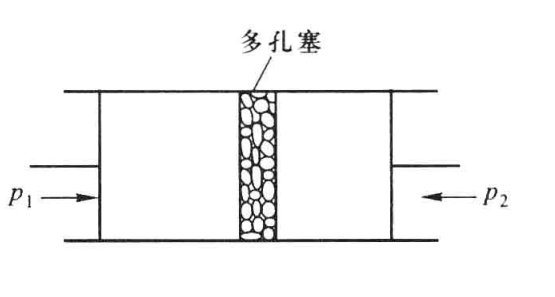
\includegraphics[width=2in]{F4.png}
		\caption{节流过程}
		\label{F4}
	\end{center}
\end{wrapfigure}
先讨论节流过程(理想气体节流过程前后温度不变)。如图2.1所示,管子多孔塞用不导热的材料包着,管子中间有一个多孔塞或节流阀.多孔塞两边各维持着较高的压强$p_1$,和较低的压强$p_2$,于是气体从高压的一边经多孔塞不断地流到低压的一边,并达到定常状态.这个过程就叫做节流过程.测量气体在多孔塞两边的温度表明,在节流过程前后,气体的温度发生了变化.这效应称为焦耳-汤姆孙效应,简称焦-汤效应,是焦耳和汤姆孙在1852年用多孔塞实验研究气体内能时发现的。\\
定义焦汤系数,其表示焓不变的情况下气体温度随压强的变化:
\begin{equation}
	\mu=(\frac{\partial T}{\partial p})_H
\end{equation}
由焓$H$可以写为$T,p$的函数$H=H(T,p)$,那么有:
\begin{equation}
	(\frac{\partial T}{\partial p})_H=-\frac{(\partial H/\partial p)_T}{(\partial H/\partial T)_p}
\end{equation}
由(\ref{x9})中$	{{C}_{p}}=(\frac{\partial H}{\partial T})_p,\quad 
	{{(\frac{\partial H}{\partial p})}_{T}}=V-T{{(\frac{\partial V}{\partial T})}_{p}} $代入到上式:
\begin{equation}
	\mu=\frac{1}{C_p}(T(\frac{\partial V}{\partial T})_p-V)=\frac{V}{C_p}(T\alpha-1)
\end{equation}
对于理想气体可知$\alpha=1/T$代入上式得$\mu=0$所以理想气体节流过程中温度不变。
\subsubsection{热辐射平衡}
\noindent
斯特藩公式:
\begin{equation}
	J_u=\frac{1}{4}caT^4=\sigma T^4
	\label{x48}
\end{equation}
$c$是光速,$a$是一个积分常量(后面会介绍),$\sigma$是斯特藩常量,约为$5.670374*10^{-8}W\cdot m^{-2} \cdot K^{-4}$。\\
空腔辐射的熵:
\begin{equation}
	S=\frac{4}{3}aT^3V
\end{equation}
可逆绝热过程中$\Delta S=0$可知$VT^3=Const$,此外平衡辐射的吉布斯函数$G=0$

我们直接给出平衡辐射(相对论情况,非相对论满足$p=\frac{2}{3}\frac{U}{V}$)中压强$p$与辐射能量密度$u$的关系(统计学可以证明):
\begin{equation}
	p=\frac{1}{3}u
	\label{x11}
\end{equation}
由空腔总的内能$U(T,V)=u(T)V$可以得到:
\begin{equation}
	u=(\frac{\partial U}{\partial V})_T=T(\frac{\partial p}{\partial T})_V-p=\frac{T}{3}\frac{\mathrm{d} u}{\mathrm{d}T}-\frac{u}{3}
\end{equation}
整理可得微分方程$T\frac{\mathrm{d}u}{\mathrm{d}T}=4u$,解得:
\begin{equation}
	u=aT^4
\end{equation}
根据辐射通量密度$J_u$与辐射内能密度$u$的关系$J_u=\frac{1}{4}cu$可以计算出斯特藩公式(\ref{x48})。\\
我们可以根据$\mathrm{d}S=\frac{\mathrm{d}U+p\mathrm{d}V}{T}$来把其熵求出:
\begin{equation}
	\mathrm{d}S=\frac{1}{T}\mathrm{d}(aT^4V)+\frac{1}{3}aT^3\mathrm{d}V=\frac{4}{3}aV\mathrm{d}T^3+\frac{4}{3}aT^3\mathrm{d}V=\mathrm{d}(\frac{4}{3}aVT^3)
\end{equation}
这样我们得到$S=\frac{4}{3}aVT^3$,没有积分常量是因为$V=0$或$T=0$时都不存在辐射场。\\
\subsubsection{电介质和磁介质的热力学理论}
\noindent
当热力学系统只包括介质不包括磁场且体积不发生变化时,功的表达式可以写为:
\begin{equation}
	\dbar W=\mu_0 \mathscr{H} V\mathrm{d}\mathscr{M}
\end{equation}
由此可以做代换:
\begin{equation}
	p \to -\mu_0\mathscr{H}\quad \quad \quad V\to V\mathscr{M}
	\label{x43}
\end{equation}
从而得到磁介质的热力学基本方程:
\begin{equation}
	\begin{split}
	\mathrm{d}U&=T\mathrm{d}S+\mu_0 \mathscr{H}V\mathrm{d}\mathscr{M}\\
	\mathrm{d}H&=T\mathrm{d}S-\mu_0V\mathscr{M}\mathrm{d}\mathscr{H}\\
	\mathrm{d}F&=-S\mathrm{d}T+\mu_0 \mathscr{H}V\mathrm{d}\mathscr{M}\\
	\mathrm{d}G&=-S\mathrm{d}T-\mu_0V\mathscr{M}\mathrm{d}\mathscr{H} 
\end{split}
\end{equation}
类似的,不考虑外电场且电介质体积不发生变化时,功可以写为:
\begin{equation}
	\dbar W=V\mathscr{E}\mathrm{d}\mathscr{D}
\end{equation}
做代换:
\begin{equation}
	p\to -\mathscr{E} \quad \quad \quad V\to V\mathscr{D}
\end{equation}	
得到电介质的热力学基本方程:
\begin{equation}
	\begin{split}
			\mathrm{d}U&=T\mathrm{d}S+ \mathscr{E}V\mathrm{d}\mathscr{D}\\
		\mathrm{d}H&=T\mathrm{d}S-V\mathscr{D}\mathrm{d}\mathscr{E}\\
		\mathrm{d}F&=-S\mathrm{d}T+ \mathscr{E}V\mathrm{d}\mathscr{D}\\
		\mathrm{d}G&=-S\mathrm{d}T-V\mathscr{D}\mathrm{d}\mathscr{E} 
	\end{split}
\end{equation}	

下面我们讨论磁致冷效应:
\begin{equation}
	(\frac{\partial T}{\partial \mathscr{H}})_S=\frac{CV}{C_{\mathscr{H}}T}\mu_0\mathscr{H} >0
\end{equation}
该式表面在熵不变(绝热可逆过程)减小磁场会使温度降低从而达到制冷的效果。\\
以$T,\mathscr{H}$为状态参量,则$S=S(T,\mathscr{H})$,那么有如下关系:
\begin{equation}
	(\frac{\partial T}{\partial \mathscr{H}})_S=-(\frac{\partial S}{\partial \mathscr{H}})_T(\frac{\partial S}{\partial T})_\mathscr{H}
	\label{x12}
\end{equation}
磁场不变时磁介质的热容为:
\begin{equation}
	C_\mathscr{H}=(\frac{\partial H}{\partial T})_\mathscr{H}=T(\frac{\partial S}{\partial T})_\mathscr{H}
	\label{x13}
\end{equation}
根据磁介质的Maxwell关系有:
\begin{equation}
	(\frac{\partial S}{\partial T})_\mathscr{H}=\mu_0 V(\frac{\partial\mathscr{M}}{\partial T})_\mathscr{H}=-\frac{\mu_0CV\mathscr{H}}{T^2}
	\label{x14}
\end{equation}	
注意上式用到了居里定律$\mathscr{M}=\frac{C}{T}\mathscr{H}$,联立(\ref{x12})(\ref{x13})(\ref{x14})即可得到$	(\frac{\partial T}{\partial \mathscr{H}})_S=\frac{CV}{C_{\mathscr{H}}T}\mu_0\mathscr{H}$。\\
理想气体绝热膨胀过程(熵不变)与其类似,也可用于制冷:
\begin{equation}
	(\frac{\partial T}{\partial p})_S=-\frac{(\partial S/\partial p)_T}{(\partial S/\partial T)_p}=\frac{T}{C_p}(\frac{\partial V}{\partial T})_p=\frac{VT\alpha}{C_p}>0
\end{equation}
\newpage
\subsection{相变}
\subsubsection{开系的热力学基本方程和热动平衡判据}
\noindent
对于开系我们需要考虑物质的量发生变化而导致的热力学基本函数发生的变化(这个变化可以认为是与物质的量成正比的量引起的),首先引入化学势:
\begin{equation}
	\mu =(\frac{\partial G}{\partial n})_{T,p}
\end{equation}
那么基本热力学函数微分形式可以写为:
\begin{equation}
	\begin{split}
		\mathrm{d}U&=T\mathrm{d}S-p\mathrm{d}V+\mu\mathrm{d}n\\
		\mathrm{d}H&=T\mathrm{d}S+V\mathrm{d}p+\mu\mathrm{d}n\\
		\mathrm{d}F&=-S\mathrm{d}T-p\mathrm{d}V+\mu\mathrm{d}n\\
		\mathrm{d}G&=-S\mathrm{d}T+V\mathrm{d}p+\mu\mathrm{d}n
	\end{split}
\label{x15}
\end{equation}	
对于吉布斯函数还有:
\begin{equation}
	G(T,p,n)=nG_m(T,p)=n\mu
\end{equation}
也就是说化学势$\mu$就等于摩尔吉布斯函数$G_m$。\\
此外还可以定义巨热力势:
\begin{equation}
	J=F-n\mu=F-G
\end{equation}
下面我们讨论热力学平衡判据,\\
\textcircled{1}对于孤立系统有熵判据$(\Delta S<0)$:
\begin{equation}
\left\{ \begin{split}
	&\delta S=0  \\
	&{{\delta }^{2}}S<0  \\
	&\delta U=\delta V=\delta N=0  \\
\end{split} \right.
\end{equation}
Tips:当$\delta^2S=0$时不能看$\delta^3S<0$,因为$\delta^3S$在引入虚变动时会有3个虚变量的乘积,不能保证正负号,因此必须保证$\delta^3S=0$,而从$\delta^4S<0$来判断,若$\delta^4S=0$则看$\delta^6S$的符号来判断,以此类推。第三行是约束条件,就是(\ref{x15})中的$\mathrm{d}$后面的变量等于0。\\
\textcircled{2}等温等体系统有自由能判据$(\Delta F>0)$:
\begin{equation}
	\left \{\begin{split}
		&\delta F=0\\
		&\delta^2F>0\\
		&\delta T=\delta V=\delta N=0
	\end{split}
\right.
\end{equation}
\textcircled{3}等温等压系统吉布斯函数判据$(\Delta G>0)$:
\begin{equation}
	\left \{\begin{split}
		&\delta G=0\\
		&\delta^2G>0\\
		&\delta T=\delta p=\delta N=0 
	\end{split}
\right.
\end{equation}
\textcircled{4}无熵变的等体系统有内能判据$(\Delta U>0)$:
\begin{equation}
	\left \{\begin{split}
		&\delta U=0\\
		&\delta^2U>0\\
		&\delta S=\delta V=\delta N=0
	\end{split}
\right.
\end{equation}
注意除了熵判据(由于熵增原理熵必须极大值才达到平衡,因此有任何扰动都会使熵减小)$\Delta S<0$其他都是大于0。\\
平衡的稳定性条件(这个证明有些trival,不想看可以跳过):
\begin{equation}
	C_V>0\quad \quad \quad (\frac{\partial p}{\partial V})_T<0
	\label{x21}
\end{equation}
这里我们利用熵判据($\delta^2S<0$)进行推导,其他判据与此等价,利用泰勒展开:
\begin{equation}
	\begin{split}
	\delta^2 S=&[(\frac{\partial^2 S}{\partial U^2})(\delta U)^2+2\frac{\partial^2 S}{\partial U\partial V}\delta U\delta V+\frac{\partial^2 S}{\partial V^2}(\delta V)^2]\\
	=&[\frac{\partial}{\partial U}(\frac{\partial S}{\partial U})_V\delta U+\frac{\partial}{\partial V}(\frac{\partial S}{\partial U})_V\delta V]\delta U+\\
	&[\frac{\partial }{\partial U}(\frac{\partial S}{\partial V})_U\delta U+\frac{\partial}{\partial V}(\frac{\partial S}{\partial V})_U\delta V]\delta V\\
	<&0
	\end{split}
\label{x18}
\end{equation}
再根据$\mathrm{d}S=\frac{1}{T}\mathrm{d}U+\frac{p}{T}\mathrm{d}V$可以得到:
\begin{equation}
	(\frac{\partial S}{\partial U})_V=\frac{1}{T}\quad \quad \quad (\frac{\partial S}{\partial V})_U=\frac{p}{T}
\end{equation}
所以(\ref{x18})可以写为:
\begin{equation}
	\delta^2S=\delta(\frac{1}{T})\delta U+\delta(\frac{p}{T})\delta V<0
	\label{x20}
\end{equation}
以$T,V$为自变量:
\begin{equation}
	\left\{\begin{split}
		&\delta U=(\frac{\partial U}{\partial T})_V\delta T+(\frac{\partial U}{\partial V})_T\delta V=C_V\delta T+[T(\frac{\partial p}{\partial T})_V-p]\delta V\\
		&\delta\frac{1}{T}=-\frac{1}{T^2}\delta T\\
		&\delta(\frac{p}{T})=\frac{1}{T^2}[T(\frac{\partial p}{\partial T})_V-p]\delta T+\frac{1}{T}(\frac{\partial p}{\partial V})_T\delta V=-\frac{1}{T^2}C_V(\delta T)^2+\frac{1}{T}(\frac{\partial p}{\partial V})_T(\delta V)^2
		\end{split}\right.
	\label{x19}
\end{equation}
把上式代入到(\ref{x20})可以得到:
\begin{equation}
	\delta^2S=-\frac{1}{T^2}C_V(\delta T)^2+\frac{1}{T}(\frac{\partial p}{\partial V})_T(\delta V)^2<0
\end{equation}
这样就得到了$C_V>0$和$(\frac{\partial p}{\partial V})_T<0$。
\subsubsection{单元系的相变}
\noindent
对于单元两相系的平衡条件(所谓单元指的是只含有一种化学成分):
\begin{equation}
	\left\{\begin{split}
			T^\alpha=T^\beta\\
			p^\alpha=p^\beta\\
			\mu^\alpha=\mu^\beta
		\end{split}
	\label{x16}
	\right.
\end{equation}
这表明整个系统达到平衡时两相的温度,压强和化学势必须分别相等,即满足热平衡、力学平衡和相变平衡。
推导过程:\\
将整个单元两相系看成一个系统可以认为是一个孤立系,那么有约束条件:
\begin{equation}
	\left\{\begin{split}
		\delta U^\alpha+\delta U^\beta =0\\
		\delta V^\alpha+\delta V^\beta=0\\
		\delta n^\alpha+\delta n^\beta=0\\
\end{split}
\right.
\end{equation}
两相熵变分别为:
\begin{equation}
	\begin{split}
		\delta S^\alpha=\frac{\delta U^\alpha+p^\alpha \delta V^\alpha-\mu^\alpha \mathrm{d}n^\alpha}{T^\alpha}\\
		\delta S^\beta=\frac{\delta U^\beta+p^\beta \delta V^\beta-\mu^\beta \mathrm{d}n^\beta}{T^\beta}
	\end{split}
\end{equation}
总熵变:
\begin{equation}
	\delta S=\delta S^\alpha+\delta S^\beta=\delta U^\alpha(\frac{1}{T^\alpha}-\frac{1}{T^\beta})+\delta V^\alpha (\frac{p^\alpha}{T^\alpha}-\frac{p^\beta}{T^\beta})-\delta n^\alpha(\frac{\mu^\alpha}{T^\alpha}-\frac{\mu^\beta}{T^\beta})=0
\end{equation}
通过上式即可得到平衡条件。如果没有达到平衡,则反应的方向都向熵增的方向进行,如$T^\alpha<T^\beta$则反应向$\delta U^\alpha>0$方向进行。\\
对于液滴,需要考虑表面相的影响(表面张力),设液滴相为$1$,蒸气相为$2$,则力学平衡条件为:
\begin{equation}
	p_1=p_2+\frac{2\sigma}{r}
\end{equation}
$\sigma$是单位长度的表面张力,量纲为$\mathrm{N\cdot m^{-1}}$。
\subsubsection{克拉珀龙方程和蒸气压方程}
\noindent
\begin{wrapfigure}[8]{r}{10em}
\begin{center}
	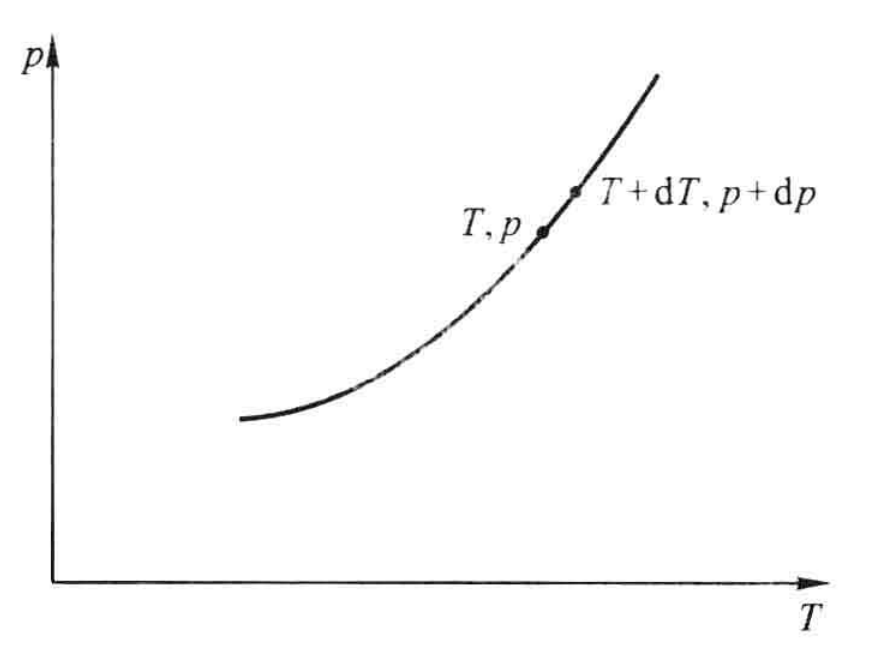
\includegraphics[width=2in]{F5.png}
	\label{F5}
\end{center}
\end{wrapfigure}
两相平衡时由于平衡条件(\ref{x16})可以得到一条平衡曲线($p$-$T$图),在平衡曲线上两相化学势相等,因此比例可以任意。这条平衡曲线满足的方程称之为克拉珀龙方程:
\begin{equation}
\frac{\mathrm{d}p}{\mathrm{d}T}=\frac{L}{T(V_m^\beta-V_m^\alpha)}
\end{equation}
式中$L$是相变潜热,代表从$\beta$相到$\alpha$相吸热的多少,根据克拉珀龙方程还可以推导出饱和气体蒸汽压方程:
\begin{equation}
	\ln p=-\frac{L}{RT}+A
\end{equation}
式中$A$是积分常量。\\
以下是推导过程:\\
首先我们知道两相平衡化学势相等$\mu^\alpha=\mu^\beta$,由于曲线上一直有这个性质,因此它们的微分也应该相等:
\begin{equation}
	\mathrm{d}\mu^\alpha=\mathrm{d}\mu^\beta
\end{equation}
根据化学势的全微分:
\begin{equation}
	\mathrm{d}\mu=\mathrm{d}G_m=-S_m\mathrm{d}T+V_m\mathrm{d}p
\end{equation}
那么就有:
\begin{equation}
	-S_m^\alpha\mathrm{d}T+V_m^\alpha\mathrm{d}p=-S_m^\beta\mathrm{d}T+V_m^\beta\mathrm{d}p
\end{equation}
整理可得:
\begin{equation}
	\frac{\mathrm{d}p}{\mathrm{d}T}=\frac{S_m^\beta-S_m^\alpha}{V_m^\beta-V_m^\alpha}
	\label{x17}
\end{equation}
由于相变时温度不发生改变,因此相变潜热可以计算为:
\begin{equation}
	L=T(S_m^\beta-S_m^\alpha)
\end{equation}
把上式代入到(\ref{x17})即可得到克拉珀龙方程$\frac{\mathrm{d}p}{\mathrm{d}T}=\frac{L}{T(V_m^\beta-V_m^\alpha)}$。\\
要计算饱和蒸汽压方程,那么可以认为气体体积远远大于液体/固体体积$(V_m^\beta>>V_m^\alpha)$,同时假定相变潜热与温度无关,再利用$pV_m=RT$,则可得到微分方程:
\begin{equation}
	\frac{1}{p}\frac{\mathrm{d}p}{\mathrm{d}T}=\frac{L}{RT^2}
\end{equation}
容易解得饱和蒸汽压方程$\ln p=-\frac{L}{RT}+A$。
\subsubsection{相变理论}	
\noindent
\textcircled{1}Maxwell等面积定则。\\
\begin{figure}[H]
\centering
\subfigure[]{
	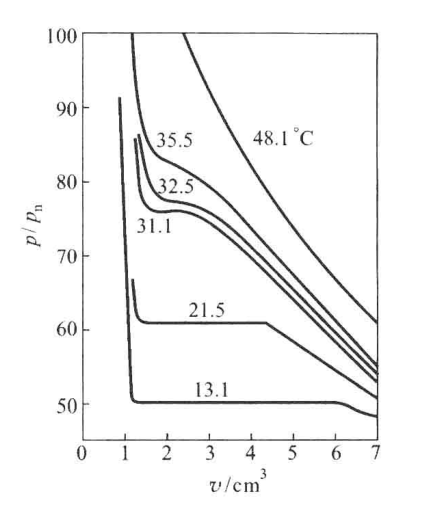
\includegraphics[scale=0.3]{F6.png} 
}
\quad\quad\quad
\subfigure[]{
	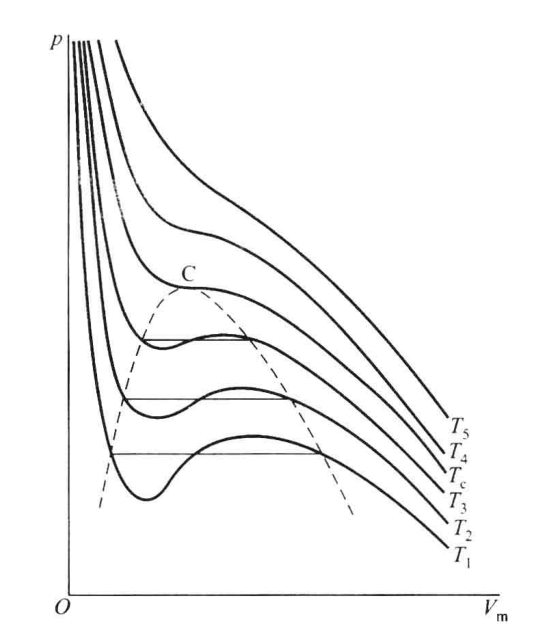
\includegraphics[scale=0.23]{F7.png}
}
\caption{实际气体等温线与范德瓦尔斯气体等温线}
\end{figure}
观察以上两图发现在高温区域气体等温线都趋近于波义耳定律给出的双曲线的形式,在低温下实际气体与范德瓦尔斯气体给出的等温线在中间部分有所差异,这一部分差异是由于相变引起的。
\begin{figure}[H]
	\centering
	\subfigure[]{
		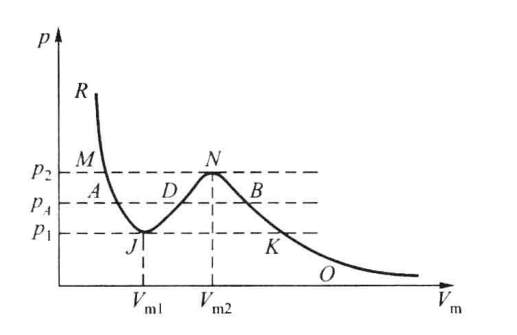
\includegraphics[scale=0.3]{F8.png} 
	}
	\quad\quad\quad
	\subfigure[]{
		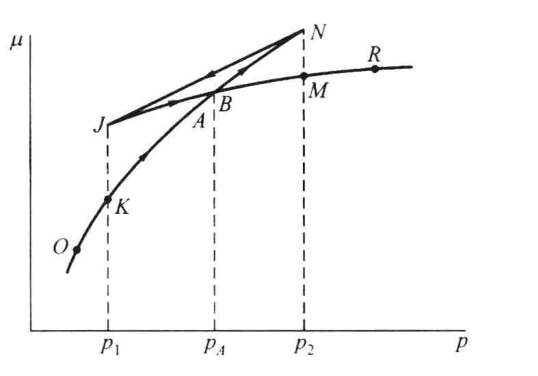
\includegraphics[scale=0.23]{F9.png}
	}
	\caption{范德瓦尔斯气体}
\end{figure}
容易看出在$J-N$过程中不满足平衡稳定性条件$(\frac{\partial p}{\partial V})_T<0$(\ref{x21})所以不可能存在,根据Maxwell等面积原理可以认为相变过程是$A-B$直线过程,其中$A-J$和$N-B$在实际中仍能出现(亚稳态),称为过热液体和过饱和蒸气。\\


\noindent
\textcircled{2}相变的分类。\\
1.非连续相变(一级相变),化学势的一级偏导数存在突变,在相变点两相化学势相等,转变时有潜热和比体积突变,在两侧化学势较低的为稳定相,较高的可以作为亚稳态存在。\\
\begin{figure}[H]
	\centering
	\subfigure[]{
		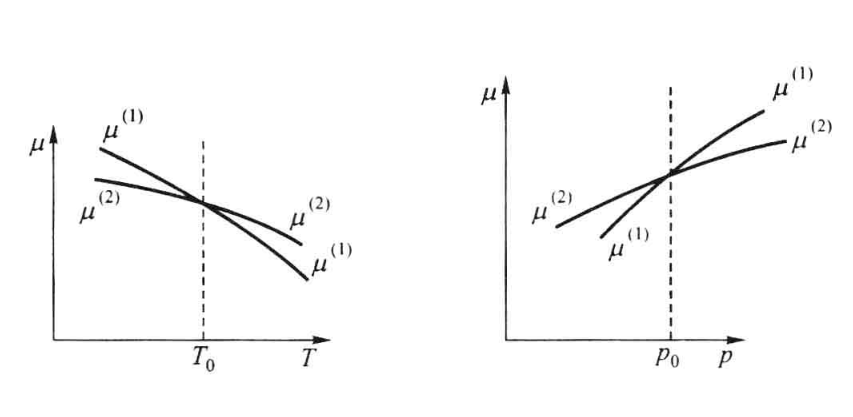
\includegraphics[scale=0.3]{F10.png} 
	}
	\quad\quad\quad
	\subfigure[]{
		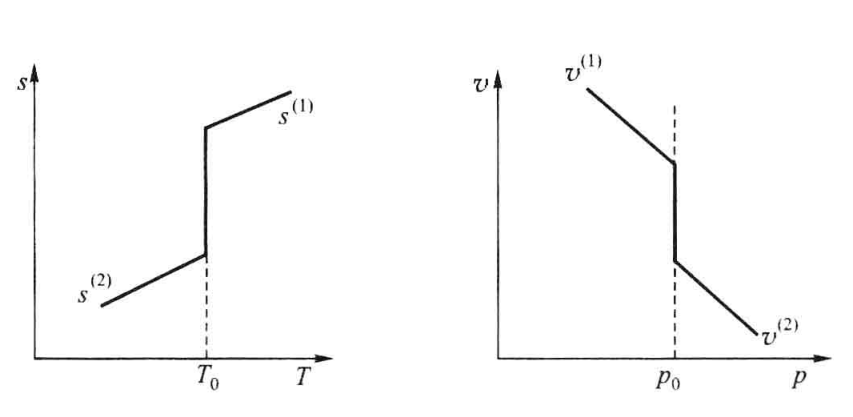
\includegraphics[scale=0.3]{F11.png}
	}
	\caption{一级相变}
\end{figure}
\noindent
2.连续相变(n级相变),化学势第n阶偏导数存在突变,在n-1阶之前一直连续,没有相变潜热和比体积突变,但是二级相变存在定压比热、定压膨胀系数和等温压缩系数的突变。\\
对于二级相变有埃伦菲斯特方程:
\begin{equation}
	\left\{\begin{split}
		&\frac{\mathrm{d}p}{\mathrm{d}T}=\frac{\alpha^{(2)}-\alpha^{(1)}}{\kappa_T^{(2)}-\kappa_T^{(1)}}\\
		&\frac{\mathrm{d}p}{\mathrm{d}T}=\frac{c_p^{(2)}-c_p^{(1)}}{Tv(\alpha^{(2)}-\alpha^{(1)})}
		\end{split}
	\right.
\end{equation}
推导过程:\\
由于二级相变化学势的一阶偏导数连续,相变点两相的比熵和比体积相等,在相变点附近的微分也相等:
\begin{equation}
	\begin{split}
		\mathrm{d}v^{(1)}=\mathrm{d}v^{(2)}\\
		\mathrm{d}s^{(1)}=\mathrm{d}s^{(2)}
	\end{split}
\end{equation}
由于:
\begin{equation}
		\mathrm{d}v=(\frac{\partial v}{\partial T})_p\mathrm{d}T+(\frac{\partial v}{\partial p})_p\mathrm{d}p=\alpha v\mathrm{d}T-\kappa_T v\mathrm{d}p
		\label{x22}
	\end{equation}
\begin{equation}
		\mathrm{d}s=(\frac{\partial s}{\partial T})_p\mathrm{d}T+(\frac{\partial s}{\partial p})_T\mathrm{d}p=\frac{c_p}{T}\mathrm{d}T-(\frac{\partial v}{\partial T})_p\mathrm{d}p=\frac{c_p}{T}\mathrm{d}T-\alpha v\mathrm{d}p
		\label{x23}
\end{equation}
根据(\ref{x22})可得:
\begin{equation}
	\begin{split}
		\alpha^{(1)}\mathrm{d}T-\kappa_T^{(1)}\mathrm{d}p&=\alpha^{(2)}\mathrm{d}T-\kappa_T^{(2)}\mathrm{d}p
		\\
		\Rightarrow \quad\quad \frac{\mathrm{d}p}{\mathrm{d}T}&=\frac{\alpha^{(2)}-\alpha^{(1)}}{\kappa_T^{(2)}-\kappa_T^{(1)}}
	\end{split}
\end{equation}
同理,根据(\ref{x23})可得:
\begin{equation}
	\begin{split}
		\frac{c_p^{(1)}}{T}\mathrm{d}T-v^{(1)}\alpha^{(1)}\mathrm{d}p&=\frac{c_p^{(2)}}{T}\mathrm{d}T-v^{(2)}\alpha^{(2)}\mathrm{d}p\\
		\Rightarrow\quad\quad
		\frac{\mathrm{d}p}{\mathrm{d}T}&=\frac{c_p^{(2)}-c_p^{(1)}}{Tv(\alpha^{(2)}-\alpha^{(1)})}
	\end{split}
\end{equation}
\begin{wrapfigure}[10]{r}{10em}
	\begin{center}
		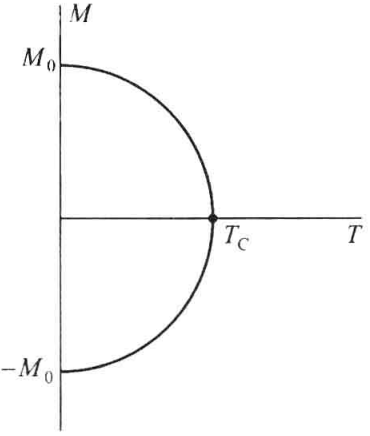
\includegraphics[width=1.5in]{F12.png}
		\label{F12}
	\end{center}
\end{wrapfigure}
\textcircled{3}朗道连续相变理论\\
对于铁磁物质其原子具有固有磁矩,两相邻原子磁矩平行时能量较低,因此在绝对零度下能量最低所有原子磁矩相互平行(有序度高),温度升高,由于热运动的存在使原子相互平行的磁矩减少(有序度降低),用$M(T)$来描述铁磁物质的有序度,$M$就是铁磁物质的自发磁矩。图中$T_C$是临界温度,超过$T_C$有序度达到最小。\\
定义朗道自由能:
\begin{equation}
	F(T,M)=F_0(T)+\frac{1}{2}a(T)M^2+\frac{1}{4}b(T)M^4+...
\end{equation}
其中$F_0(T)$是$M=0$时的自由能,由于系统对于$M$和$-M$是等价的,因此没有奇数幂项。\\
下面我们给出$T>T_c$(a)和$T<T_c$(b)的朗道自由能曲线:
\begin{figure}[H]
	\centering
		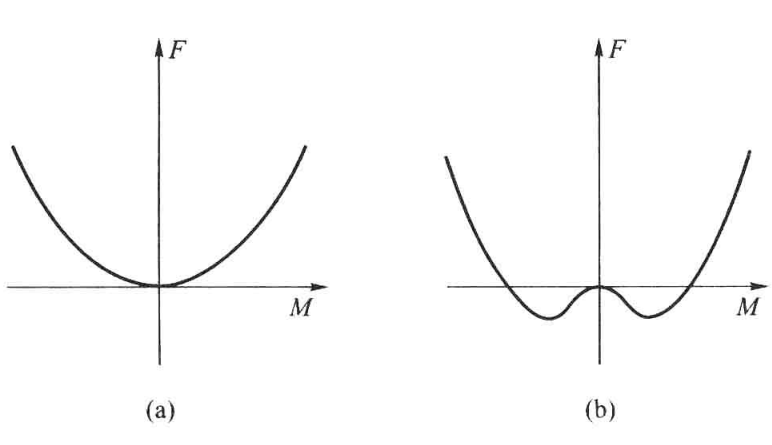
\includegraphics[scale=0.3]{F13.png}
		\caption{朗道自由能}
\end{figure}
自由能取值分别为:
\begin{equation}
	\left\{\begin{split}
	&F=F_0,&(T>T_c)	\\
	&F=F_0-\frac{a^2}{4b},&(T<T_c)
	\end{split}\right.
\end{equation}
推导:\\
在$F$取极值时,有(稳定平衡态应该取极小值,所以二阶导大于0):
\begin{equation}
		\frac{\partial F}{\partial M}=M(a+bM^2)=0
	\end{equation}
\begin{equation}
		\frac{\partial^2 F}{\partial M^2}=a+3bM^2>0
		\label{x24}
\end{equation}
只考虑取极值$(\frac{\partial F}{\partial M})=0$有三个解:
\begin{equation}
	M=0,M=\pm \sqrt{-\frac{a}{b}}
\end{equation}
$M=0$代表无序态,对应于$T>T_c$,将$M=0$代入到(\ref{x24})中可以得到$a>0$;$T<T_C$时,将$M=\pm \sqrt{-a/b}$代入(\ref{x24})可以得到$a<0$,由此可以推断出在$T=T_c$时$a=0$.\\
由此可以得知$T>T_c$有$a>0,b>0$,$F=F_0$; $T<T_c$有$a<0,b>0$,$F=F_0-\frac{a^2}{4b}$.


\subsubsection{多元系相变}
\noindent
对于多元系一般认为体积$V$,内能$U$,熵$S$和吉布斯函数$G$都是各组元物质的量的一次齐函数:
\begin{equation}
	\left\{\begin{split}
		&V=\sum n_i(\frac{\partial V}{\partial n_i})_{T,p,n_j}&=\sum n_i v_i\\
		&U=\sum n_i(\frac{\partial U}{\partial n_i})_{T,p,n_j}&=\sum n_iu_i\\
		&S=\sum n_i (\frac{\partial S}{\partial n_i})_{T,p,n_j}&=\sum n_is_i\\
		&G=\sum n_i (\frac{\partial G}{\partial n_i})_{T,p,n_j}&=\sum n_i\mu_i		
	\end{split}\right.
\end{equation}	
其中$v_i,u_i,s_i$分别表示$i$组元的摩尔体积,摩尔内能,摩尔熵	,$\mu_i$是组元$i$的化学势。\\
多元系的复相平衡条件:
\begin{equation}
	\mu_i^\alpha=\mu_i^\beta
\end{equation}
其中设两相$\alpha$和$\beta$都有$k$个组元,上式表示$k$个组元中任意组元$i$在两相的化学势相等。(这里的组元意思是同一种化学物质,例如水和氧气组成的多元系有2个组元,液相$\mathrm{H_2O}$和气相$\mathrm{H_2O}$是不同相的同一组元,对于上式的意思就是液相中水的化学势等于气相中水的化学势,但不一定等于$\mathrm{O_2}$的化学势。)\\
推导:在不发生化学反应的情况下,$i$组元在两相中物质的量不变,有:
\begin{equation}
	\delta n_i^\alpha+\delta n_i^\beta=0
\end{equation}	
总吉布斯函数的变化为:
\begin{equation}
	\delta G=\delta G^\alpha+\delta G^\beta=\sum u_i^\alpha \delta n_i^\alpha+\sum u_i^\beta n_i^\beta=\sum (\mu_i^\alpha-\mu_i^\beta)\delta n_i^\alpha
\end{equation}
达到平衡态时有$\delta G=0$因此$\mu_i^\alpha=\mu_i^\beta$	.\\

\noindent
吉布斯相律,对于$\varphi$个相,$k$个组元的独立参数的个数为:
\begin{equation}
	f=k+2-\varphi
\end{equation}
\subsubsection{混合理想气体}
\noindent
理想溶液中$i$组元的化学势:
\begin{equation}
	\mu_i=g_i(T,p)+RT\ln x_i
\end{equation}	
$g_i$是纯$i$组元的化学势,$x_i$是溶液中$i$组元的摩尔分数。\\
混合理想气体各组元分压与总压的关系:
\begin{equation}
	p=\underset{i}{\sum}p_i\quad\quad\quad p_i=x_ip 
\end{equation}	
理想气体化学平衡:
\begin{equation}
	\underset{i}{\sum}v_i \mu_i=0
\end{equation}
其中$v_i$是化学反应式$\underset{i}{\sum}v_i A_i=0$中组元$i$的配平系数(注意可正可负)。
\subsubsection{热力学第三定律}	
\noindent
	1.能斯特定理:凝聚系的熵在等温过程中的改变随热力学温度趋于0。($ \underset{T\to 0}{\mathop{\lim }}\,{{(\Delta S)}_{T}}=0$)\\
	2.绝对零度不能达到原理不可能通过有限步骤使一个物体冷却到热力学温度零度。\\
	3.$\underset{T\to 0}{\mathrm{lim}}S_0=0$:$T\to 0K$时,同一物质处在热力学平衡的一切形态具有相同的熵。
	\\
其中能斯特定理可以推广到在$T\to 0$时物质的熵与任意状态参量$y$的数值无关:
\begin{equation}
	S(0,y_A)=S(0,y_B)
\end{equation}

\noindent 根据能斯特定律可以证明如下结论(其中后两个用到了Maxwell关系):\\
当$T \to 0$时,有:
\begin{equation}
	\left \{
	\begin{split}
	&C_y=T(\frac{\partial S}{\partial T})_y=(\frac{\partial S}{\partial \ln T})_y=0\\
	&\underset{T\to 0}{\lim}(\frac{\partial V}{\partial T})_p=-(\frac{\partial S}{\partial p})_T=0\\
	&\underset{T\to 0}{\lim}(\frac{\partial p}{\partial T})_V=(\frac{\partial S}{\partial V})_T=0		
	\end{split}\right.
\end{equation}
根据$\underset{T\to 0}{\lim}S=0$可以得到:
\begin{equation}
	S(T,p)=\int_{0}^{T} \frac{C_p(T,p)}{T}\mathrm{d}T
\end{equation}
若过程中发生相变,则有:
\begin{equation}
	S(T,p)=\int_{0}^{T_0} \frac{C_p(T,p)}{T}\mathrm{d}T+\frac{L}{T_0}+\int_{T_0}^{T} \frac{C_p'(T,p)}{T}\mathrm{d}T
\end{equation}
其中$T_0$是相变温度,$C_p$是固相的定压热容,$C_p'$是相变后的定压热容。
\newpage
\section{统计物理}
\subsection{近独立粒子的统计分布}
\subsubsection{粒子运动状态的量子描述}
\noindent
\textcircled{1}谐振子:
\begin{equation}
	\varepsilon_n=\hbar \omega(n+\frac{1}{2})
	\label{x42}
\end{equation}
\textcircled{2}转子:
\begin{equation}
	\varepsilon_l=\frac{l(l+1)\hbar^2}{2I}
\end{equation}
\textcircled{3}电子自旋:
\begin{equation}
	\varepsilon =-\vec{\mu }\cdot \vec{B}=\pm \frac{e \hbar}{2m}B
\end{equation}
\textcircled{4}自由粒子:
\begin{equation}
	\varepsilon=\frac{2\pi^2\hbar^2}{m}\frac{n_x^2+n_y^2+n_z^2}{L^2}
\end{equation}
自由粒子的推导,先讨论一维无限深势阱,设自由粒子在$0<x<L$内的无线深势阱中,则仅需求解定态薛定谔方程:
\begin{equation}
	\left \{
	\begin{split}
		&\hat{H}\psi(x)=E\psi(x)\\
		&V(x)=0\quad \quad (0<x<L)\\
		&V(x)=\infty \quad\quad x=others
	\end{split}\right.
\end{equation}
在$0<x<L$时,有:
\begin{equation}
	-\frac{\hbar^2}{2m}\frac{\partial^2 \psi}{\partial x^2}=E\psi
\end{equation}
令$k=\sqrt{2mE}/\hbar$,则可以解出:
\begin{equation}
	\psi(x)=A\sin kx+B\cos kx
\end{equation}
再根据边界条件$\psi(0)=\psi(L)=0$可以得出$B=0$, $k_n=n\pi/L$,这样可以解出:
\begin{equation}
	E_n=\frac{n^2\pi^2\hbar^2}{2mL^2}
\end{equation}
拓展到三维,设自由粒子(有2个运动方向,要乘一个2)在$0<x<L,0<y<L,0<z<L$的无限深势阱中,由$\varepsilon_{n_x}=p_x^2/2m=\frac{2\pi^2\hbar^2}{m}\frac{n_x^2}{L^2}$可以计算出:
\begin{equation}
	\left\{\begin{split}
		p_x=\frac{h}{L}n_x\\
		p_y=\frac{h}{L}n_y\\
		p_z=\frac{h}{L}n_z
	\end{split}\right.
\end{equation}
再根据$\varepsilon=(p_x^2+p_y^2+p_z^2)/2m$可以求出$\varepsilon=\frac{2\pi^2\hbar^2}{m}\frac{n_x^2+n_y^2+n_z^2}{L^2}$。

\noindent
在体积$V$内,在$\varepsilon \sim \varepsilon+\mathrm{d}\varepsilon$范围内的自由粒子可能的状态数为:
\begin{equation}
	D(\varepsilon)\mathrm{d}\varepsilon=\frac{2\pi V}{h^3}(2m)^{3/2}\varepsilon^{1/2}\mathrm{d}\varepsilon
\end{equation}
推导过程:\\
在三维情况下自由粒子状态数由$n_x,n_y,n_z$表征,设能量为准连续的,考虑$V=L^3$内的自由粒子运动,则有:
\begin{equation}
	\mathrm{d}n_i=\frac{L}{h}\mathrm{d}p_i\quad\quad\quad(i=x,y,z)
\end{equation}
那么在$p_x\sim p_x+\mathrm{d}p_x, p_y\sim p_y+\mathrm{d}p_y, p_z\sim p_z+\mathrm{d}p_z$范围内可能的粒子状态数为:
\begin{equation}
	\mathrm{d}n_x\mathrm{d}n_y\mathrm{d}n_z=\frac{V}{h^3}\mathrm{d}p_x\mathrm{d}p_y\mathrm{d}p_z
\end{equation}
转换为球坐标系中,由于$\theta$和$\varphi$的对称性,则在动量大小$p\sim p+\mathrm{d}p$的球壳内的可能的粒子状态数为:
\begin{equation}
	\frac{4\pi V}{h^3}p^2\mathrm{d}p
	\label{x49}
\end{equation}
由$\varepsilon=p^2/2m$可知$m\mathrm{d}\varepsilon=p\mathrm{d}p$,则有在$\varepsilon\sim \varepsilon+\mathrm{d}\varepsilon$范围内的自由粒子状态数:
\begin{equation}
	D(\varepsilon)\mathrm{d}\varepsilon=\frac{4\pi V}{h^3}\cdot 2m\varepsilon\cdot \frac{m}{\sqrt{2m\varepsilon}}\mathrm{d}\varepsilon=\frac{2\pi V}{h^3}(2m)^{3/2}\varepsilon^{1/2}\mathrm{d}\varepsilon
	\label{x40}
\end{equation}
\subsubsection{分布和微观状态}
对于由粒子数为$N$,能量为$E$,体积为$V$的全同粒子组成的系统:\\
能级:
\[\varepsilon_1, \varepsilon_2, ..., \varepsilon_l,...\]
简并度:
\[\omega_1, \omega_2,..., \omega_l,...\]
粒子数:
\[a_1, a_2,..., a_l,...\]
对于玻尔兹曼系统,粒子可以分辨,则每一层能级上可能的状态数为$\omega_l^{a_l}$(每个粒子都有$\omega_l$个选择,一层能级上有$a_l$个粒子),由于粒子可以分辨,则$N$个粒子间两两交换仍然成立,因此可以有因子$N!$,但是在各个能级间已经交换过粒子数了,所以再除以每各能级的交换数$a_l!$,可以得到分布$\{a_l\}$对应的微观状态数为:
\begin{equation}
	\Omega_{M.B}=\frac{N!}{\prod\limits_{l}{{{a}_{l}}!}}\prod_{l} \omega_l^{a_l}
	\label{x25}
\end{equation}
\begin{wrapfigure}[3]{r}{10em}
	\begin{center}
		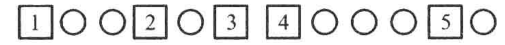
\includegraphics[width=2in]{F14.png}
		\label{F14}
	\end{center}
\end{wrapfigure}
对于玻色系统,粒子不可分辨,不遵守Pauli不相容原理,因此每个能级有$C_{\omega_l+a_l-1}^{a_l}$个状态数(如右图,可以把圆圈视为粒子,在矩形右边代表在该简并度的粒子数,右图中一共7个粒子,在5个简并度中的分布),则分布$\{a_l\}$对应的微观状态数为:
\begin{equation}
	\Omega_{B.E}=\prod_{l}C_{\omega_l+a_l-1}^{a_l}=\prod_{l} \frac{(\omega_l+a_l-1)!}{a_l! (\omega_l-1)!}
	\label{x32}
\end{equation}
对于费米系统,粒子不可分辨,遵守Pauli不相容原理,因此每个能级有$C_{\omega_l}^{a_l}$个状态数,则分布$\{a_l\}$对应的微观状态数为:
\begin{equation}
	\Omega_{F.D}=\prod_{l} C_{\omega_l}^{a_l}=\prod_{l}\frac{\omega_l!}{a_l!(\omega_l-a_l)!}
	\label{x33}
\end{equation}
三种分布的关系:\\
当满足非简并条件(经典极限条件):	
	\begin{equation}
		\frac{a_l}{\omega_l}\ll 1
	\end{equation}
有如下关系:
\begin{equation}
	\Omega_{B.E}=\Omega_{F.D}=\frac{\Omega_{M.B}}{N!}
\end{equation}
	\newpage
\subsection{最概然分布的三个统计}
	\subsubsection{Boltzmann分布}
\noindent
Boltzmann 分布的表达式:
\begin{equation}
		a_l=\omega_l \mathrm{e}^{-\alpha-\beta \varepsilon_l}
\end{equation}
其中$\alpha, \beta$由约束条件确定:
\begin{equation}
	N=\sum_{l}\omega_l \mathrm{e}^{-\alpha-\beta \varepsilon_l}\quad\quad E=\sum_{l}\omega_l\varepsilon_l \mathrm{e}^{-\alpha-\beta \varepsilon_l}
\end{equation}
推导:\\
对Maxwell-Boltzmann微观状态数$\Omega_{M.B}$(\ref{x25})取对数:
\begin{equation}
	\ln \Omega_{M.B}=\ln \frac{N!}{\prod_{l} a_l!}\prod_{l}\omega_l^{a_l}
\end{equation}
利用近似等式$\ln m!=m(\ln m-1)$(这个推导有一个缺陷,就是实际上$a_l$并非总是远远大于1的):
\begin{equation}
	\begin{split}
	\ln \Omega_{M.B}&=N(\ln N-1)-\sum_{l}  a_l(\ln a_l-1)+\sum_l a_l\ln \omega_l\\
	&=N\ln N-\sum_{l}a_l\ln a_l+\sum_{l}a_l\ln \omega_l
	\end{split}
	\label{x31}
\end{equation}
当$\ln \Omega_{M.B}$达到极大值分布时($\delta \Omega_{M.B}=0$)也可以认为$\Omega_{M.B}$达到极大值,对$\ln \Omega_{M.B}$取变分,有:
\begin{equation}
	\delta \Omega_{M.B}=-\sum_{l} \delta a_l \ln a_l-\sum_{l} \delta a_l +\sum_{l}a_l\ln \omega_l=-\sum_{l} \ln \frac{a_l}{\omega_l}\delta a_l
\end{equation}
此时取得的极值并不能保证满足约束条件$(\delta N=\sum_{l}\delta a_l =0, \delta E=\delta a_l \varepsilon_l=0)$,为此我们引入$\alpha,\beta$两个参量,利用拉格朗日乘子法:
\begin{equation}
	\delta \ln \Omega_{M.B}-\alpha \delta N-\beta E=-\sum_{l}(\ln \frac{a_l}{\omega_l}+\alpha+\beta \varepsilon_l)\delta a_l=0
\end{equation}
所以有:
\begin{equation}
	\ln \frac{a_l}{\omega_l}+\alpha+\beta \varepsilon_l=0
	\label{x30}
\end{equation}
即$a_l=\omega_l\mathrm{e}^{-\alpha-\beta \varepsilon_l}$.
\subsubsection{Boltzmann分布热力学量的统计表达式}
\noindent
引入配分函数(自变量为$\beta, y$):
\begin{equation}
	Z_1=\sum_{l} \omega_l \mathrm{e}^{-\beta \varepsilon_l}
\end{equation}
则有内能:
\begin{equation}
		U=-N\frac{\partial}{\partial \beta}\ln Z_1
		\label{x26}
	\end{equation}
广义力:
\begin{equation}
		Y=-\frac{N}{\beta}\frac{\partial}{\partial y}\ln Z_1
		\label{x27}
\end{equation}
熵:
	\begin{equation}
		S=k\ln \Omega_{M.B}
		\label{x28}
	\end{equation}

\noindent
首先对内能(\ref{x26})进行推导:\\
内能是系统中粒子无规则运动的统计平均值,所以有
\begin{equation}
	U=\sum_l a_l \varepsilon_l =\sum_l \varepsilon_l \mathrm{e}^{-\alpha-\beta \varepsilon_l}
\end{equation}
由$N=\mathrm{e}^{-\alpha}Z_1$可得:
\begin{equation}
	U=\mathrm{e}^{-\alpha} \sum_{l} \varepsilon_l \omega_l \mathrm{e}^{-\beta \varepsilon_l}=\frac{N}{Z_1}(-\frac{\partial}{\partial \beta})Z_1=-N\frac{\partial}{\partial \beta}\ln Z_1
\end{equation}
广义力(\ref{x27})的推导:\\
外界对系统的广义力(能量对广义坐标的偏导数)为:
\begin{equation}
	\begin{split}
	Y&=\sum_{l}\frac{\partial \varepsilon_l}{\partial y}a_l=\sum_l \frac{\partial \varepsilon_l}{\partial y}\mathrm{e}^{-\alpha-\beta \varepsilon_l}\\
	&=\mathrm{e}^{-\alpha} (-\frac{1}{\beta} \frac{\partial}{\partial y}) \sum_{l} \omega_l \mathrm{e}^{-\beta\varepsilon_l}\\
	&=\frac{N}{Z_1}(-\frac{1}{\beta} \frac{\partial}{\partial y})Z_1\\
	&=-\frac{N}{\beta}\frac{\partial}{\partial y}\ln Z_1
	\end{split}
\end{equation}
熵(\ref{x28})的推导:\\
由热力学基本方程$\mathrm{d}U=T\mathrm{d}S+Y\mathrm{d}y$,所以
\begin{equation}
\begin{split}
	\mathrm{d}S&=\frac{1}{T}(\mathrm{d}U-Y\mathrm{d}y)\\
	&=\frac{1}{T}[-N\mathrm{d}(\frac{\partial }{\partial \beta}\ln Z_1)+\frac{N}{\beta} \frac{\partial}{\partial y} \ln Z_1 \mathrm{d}y]
\end{split}
\end{equation}
 将上式两边同乘$\beta$可得:
\begin{equation}
	\begin{split}
		\beta \mathrm{d}S&=\frac{N}{T}[-\beta\mathrm{d}\frac{\partial \ln Z_1}{\partial \beta}+\frac{\partial}{\partial y}\ln Z_1\mathrm{d}y]
		\\
		\beta \dbar Q&=N[-\beta\mathrm{d}\frac{\partial \ln Z_1}{\partial \beta}+\frac{\partial}{\partial y}\ln Z_1\mathrm{d}y]
		\label{x29}
		\end{split}
\end{equation}
由配分函数的全微分:
\begin{equation}
	\mathrm{d}\ln Z_1=\frac{\partial \ln Z_1}{\partial \beta}\mathrm{d}\beta +\frac{\partial \ln Z_1}{\partial y}\mathrm{d}y
\end{equation}
所以有:
\begin{equation}
	\begin{split}
	\mathrm{d}[\ln Z_1-\beta \frac{\partial}{\partial \beta}(\ln Z_1)]&=\frac{\partial \ln Z_1}{\partial \beta}\mathrm{d}\beta +\frac{\partial \ln Z_1}{\partial y}\mathrm{d}y-\frac{\partial}{\partial \beta}\ln Z_1\mathrm{d}\beta-\beta \mathrm{d}\frac{\partial}{\partial \beta}\ln Z_1\\
	&=\frac{\partial \ln Z_1}{\partial y}\mathrm{d}y-\beta \mathrm{d}\frac{\partial}{\partial \beta}\ln Z_1
	\end{split}
\end{equation}
由$T$和$\beta$都是$\dbar Q$的积分因子,可以令$\beta=1/kT$,把上式代入到(\ref{x29})可得:
\begin{equation}
	\mathrm{d}S=Nk\mathrm{d}(\ln Z_1-\beta \frac{\partial }{\partial \beta}\ln Z_1)
\end{equation}
积分并取积分常数为0,得到:
\begin{equation}
	S=Nk(\ln Z_1-\beta \frac{\partial }{\partial \beta}\ln Z_1)
\end{equation}
由$\ln Z_1=\ln N+\alpha$,所以:
\begin{equation}
	\begin{split}
		S&=k(N\ln N+\alpha N+\beta U)\\
		&=k[N\ln N+\sum_{l}(\alpha +\beta \varepsilon_l)a_l]
	\end{split}
\end{equation}
再根据$\ln \frac{a_l}{\omega_l}+\alpha+\beta \varepsilon=0$(\ref{x30})以及$\ln \Omega_{M.B}=N\ln N-\sum a_l\ln a_l+\sum a_l\ln \omega_l$(\ref{x31})可得:
\begin{equation}
	S=k(N\ln N+\sum_l a_l\ln \omega_l-\sum_l a_l \ln a_l)=k\ln \Omega_{M.B}
\end{equation}
\subsubsection{Bose分布}
\noindent
Bose分布的表达式:
\begin{equation}
	a_l=\frac{\omega_l}{\mathrm{e}^{\alpha +\beta \varepsilon_l}-1}
\end{equation}
其中$\alpha$,$\beta$由约束条件确定:
\begin{equation}
	N=\sum_{l} \frac{\omega_l}{\mathrm{e}^{-\alpha+\beta\varepsilon_l}-1}\quad\quad E=\sum_{l} \frac{ \omega_l \varepsilon_l}{ \mathrm{e}^{\alpha+\beta\varepsilon_l}-1}
\end{equation}
推导:\\
对Bose-Eunstein分布$\Omega_{B.E}$(\ref{x32})取对数, 并利用近似等式$\ln m!=m(\ln m-1)$,设$a_l\gg 1, \omega_l\gg 1$(前面说的$a_lgg1$的缺陷仍然存在),则有$ w_l+a_l-1 \simeq \omega_l+a_l, \omega_l-1\simeq \omega_l$:
\begin{equation}
	\begin{split}
	\ln \Omega_{B.E}&=\sum_{l} \ln \frac{(\omega_l+a_l-1)!}{a_l! (\omega_l-1)!}\\
	&=\sum_{l} [\ln(\omega_l+a_l-1)!-\ln a_l!-\ln (\omega_l-1)!]\\
	&=\sum_{l} [(\omega_l+a_l)\ln(\omega_l+a_l)-a_l\ln a_l - \omega_l \ln \omega_l]
\end{split}
\end{equation}
对$a_l$取变分,当$\ln \Omega_{B.E}$取极大值时必有$\delta \ln \Omega_{B.E}=0$:
\begin{equation}
	\delta \ln \Omega_{B.E}=\sum_l [\ln (\omega_l+a_l)-\ln a_l-1]\delta a_l=\sum_l [\ln (\omega_l+a_l)-\ln a_l]\delta a_l=0
\end{equation}
要保证满足约束条件$\delta N=\sum_l \delta a_l =0, \delta E=\sum_{l} \varepsilon_l \delta a_l=0$,使用拉格朗日乘子法,引入$\alpha, \beta$:
\begin{equation}
	\delta \ln \Omega_{B.E}= \sum_l [\ln (\omega_l+a_l)-\ln a_l-\alpha -\beta \varepsilon_l]=0
\end{equation}
由此可得:
\begin{equation}
	\ln (\frac{\omega_l+a_l}{a_l})-\alpha-\beta \varepsilon_l=0
\end{equation}
整理可得$a_l=\frac{\omega_l}{\mathrm{e}^{\alpha+\beta \varepsilon_l}-1}$ .
\subsubsection{Bose分布热力学量的统计表达式}
\noindent
引入巨配分函数(自变量为$\alpha, \beta, y$):
\begin{equation}
	\Xi = \prod_l \Xi_l =\prod_l (1-\mathrm{e}^{-\alpha-\beta \varepsilon_l})^{-\omega_l}
\end{equation}
其对数为:
\begin{equation}
	\ln \Xi=-\sum_l \omega_l \ln (1-\mathrm{e}^{-\alpha-\beta \varepsilon_l}) 
\end{equation}
那么系统的平均总粒子数:
\begin{equation}
	\bar{N}=-\frac{\partial}{\partial \alpha}\ln \Xi
\end{equation}
内能:
\begin{equation}
	\begin{split}
		U&=\sum_l a_l=\sum_l \frac{\varepsilon_l \omega_l}{\mathrm{e}^{\alpha+\beta \varepsilon_l}-1}\\
		&=-\frac{\partial }{\partial \beta}\ln \Xi
	\end{split}
\end{equation}
广义力:
\begin{equation}
	\begin{split}
		Y&=\sum_l \frac{\partial \varepsilon_l}{\partial y} a_l=\sum_l \frac{\omega_l}{\mathrm{e}^{\alpha+\beta \varepsilon_l}-1}\frac{\partial \varepsilon_l}{\partial y}\\
		&=\sum_l\omega_l \frac{\partial}{\partial y}\ln (1-\mathrm{e}^{-\alpha-\beta \varepsilon_l}) \\
		&=-\frac{1}{\beta}\frac{\partial}{\partial y}\ln \Xi
	\end{split}
\end{equation}
熵:
\begin{equation}
	S=k\ln \Omega_{B.E}
\end{equation}
\subsubsection{Fermi分布}
\noindent
Feimi分布的表达式:
\begin{equation}
	a_l=\frac{\omega_l}{\mathrm{e}^{\alpha +\beta \varepsilon_l}+1}
\end{equation}
其中$\alpha$,$\beta$由约束条件确定:
\begin{equation}
	N=\sum_{l} \frac{\omega_l}{\mathrm{e}^{-\alpha+\beta\varepsilon_l}+1}\quad\quad E=\sum_{l} \frac{ \omega_l \varepsilon_l}{ \mathrm{e}^{\alpha+\beta\varepsilon_l}+1}
\end{equation}
推导:\\
对Fermi-Dirac分布$\Omega_{B.E}$(\ref{x32})取对数, 并利用近似等式$\ln m!=m(\ln m-1)$,设$a_l\gg 1, \omega_l\gg 1$(前面说的$a_l\gg1$的缺陷仍然存在),$\omega_l-a_l\gg l$, 则有:
\begin{equation}
	\begin{split}
		\ln \Omega_{F.D}&=\sum_l\ln\frac{\omega_l!}{(\omega_l-a_l)! a_l!} 
		\\
		&=\sum_l [\ln \omega_l!-\ln a_l!-\ln(\omega_l-a_l)!]
		\\
		&=\sum_{l}[\ln \omega_l \ln \omega_l -a_l\ln a_l-(\omega_l-a_l)\ln (\omega_l-a_l)]
	\end{split}
\end{equation}
对$a_l$取变分,当$\ln \Omega_{F.D}$取极大值时必有$\delta \ln \Omega_{F.D}=0$:
\begin{equation}
	\delta \ln \Omega_{F.D}=-\sum_l [\ln a_l -\ln (\omega_l-a_l)]\delta a_l
\end{equation}
要保证满足约束条件$\delta N=\sum_l \delta a_l =0, \delta E=\sum_{l} \varepsilon_l \delta a_l=0$,使用拉格朗日乘子法,引入$\alpha, \beta$:
\begin{equation}
	\delta \ln \Omega_{F.D}= \sum_l [\ln (\omega_l-a_l)-\ln a_l-\alpha -\beta \varepsilon_l]\delta a_l=0
\end{equation}
由此可得:
\begin{equation}
	\ln (\frac{\omega_l-a_l}{a_l})-\alpha-\beta \varepsilon_l=0
\end{equation}
整理可得$a_l=\frac{\omega_l}{\mathrm{e}^{\alpha+\beta \varepsilon_l}+1}$ .
\subsubsection{Fermi分布热力学量的统计表达式}
\noindent
引入巨配分函数(自变量为$\alpha, \beta, y$):
\begin{equation}
	\Xi = \prod_l \Xi_l =\prod_l (1+\mathrm{e}^{-\alpha-\beta \varepsilon_l})^{\omega_l}
\end{equation}
其对数为:
\begin{equation}
	\ln \Xi=\sum_l \omega_l \ln (1+\mathrm{e}^{-\alpha-\beta \varepsilon_l}) 
\end{equation}
那么系统的平均总粒子数:
\begin{equation}
	\bar{N}=-\frac{\partial}{\partial \alpha}\ln \Xi
\end{equation}
内能:
\begin{equation}
	\begin{split}
		U&=\sum_l a_l=\sum_l \frac{\varepsilon_l \omega_l}{\mathrm{e}^{\alpha+\beta \varepsilon_l}+1}\\
		&=-\frac{\partial }{\partial \beta}\ln \Xi
	\end{split}
\end{equation}
广义力:
\begin{equation}
	\begin{split}
		Y&=\sum_l \frac{\partial \varepsilon_l}{\partial y} a_l=\sum_l \frac{\omega_l}{\mathrm{e}^{\alpha+\beta \varepsilon_l}+1}\frac{\partial \varepsilon_l}{\partial y}\\
		&=\sum_l\omega_l \frac{\partial}{\partial y}\ln (1+\mathrm{e}^{-\alpha-\beta \varepsilon_l}) \\
		&=-\frac{1}{\beta}\frac{\partial}{\partial y}\ln \Xi
	\end{split}
\end{equation}
熵:
\begin{equation}
	S=k\ln \Omega_{F.D}
\end{equation}

\newpage
\subsection{系综理论}
\subsubsection{刘维尔定理}
\noindent
刘维尔定理:\begin{equation}
	\frac{\mathrm{d} \rho}{\mathrm{d}t}=0
\end{equation}
$\rho(q_i,p_i,t)$为系统的代表点在相空间某点出现的概率,刘维尔定理也可以写为:
\begin{equation}
	\frac{\partial \rho}{\partial t}=-[\rho, H]
\end{equation}
其中$[\rho , H]$表示泊松括号,即:
\begin{equation}
	[\rho, H]=\sum_i (\frac{\partial \rho}{\partial q_i}\frac{\partial H}{\partial p_i}-\frac{\partial \rho}{\partial p_i}\frac{\partial H}{\partial q_i})
\end{equation}
证明过程:\\
首先我们引入系综的概念,系综就是指近乎无穷多个与所研究的系统完全相同又互不影响的的系统的集合,若系统自由度为$f=Nr$($N$个粒子,每个粒子具有$r$个自由度),那么可以用$f$个广义坐标$(q_1,q_2,...,q_f)$和$f$个广义动量$(p_1,p_2,...,p_f)$来描述系统,相空间就是一个$2f$维空间,系统在其中可以用一个点表示,一般来说我们研究的系统都是孤立系统,使用系统的哈密顿量$H$应该是确定的,根据分析力学的理论可以知道系统代表点在相空间的轨迹总是符合正则方程:
\begin{equation}
\left\{\begin{split}
	\frac{\partial H}{\partial q_i}&=-\dot{p_i}\\
	\frac{\partial H}{\partial p_i}&=\dot{q_i}\quad\quad\quad (i=1,2,...,f)
\end{split}\right.
\end{equation}
我们可以认为系综的系统量是守恒的,也就是系统的代表点数量是守恒的,那么可以利用连续性方程(\ref{x35}):
\begin{equation}
	\begin{split}
	\frac{\partial \rho}{\partial t}&=-\nabla \cdot (\rho \mathbf{v})=-\nabla\rho\cdot(\dot{q_1},\dot{q_2},...,\dot{q_f};\dot{p_1},\dot{p_2},...,\dot{p_f})-\rho \cdot \nabla \mathbf{v}\\
	&=-[\sum_i \frac{\partial \rho}{\partial q_i}\dot{q_i}+\sum_i\frac{\partial \rho}{\partial p_i}\dot{p_i}+\rho(\sum_i \frac{\partial \dot{q_i}}{\partial q_i}+\sum_i \frac{\partial \dot{p_i}}{\partial p_i})]\\
	&=-[
	\sum_i (\frac{\partial \rho}{\partial q_i}\frac{\partial H}{\partial p_i}-\frac{\partial \rho}{\partial p_i}\frac{\partial H}{\partial q_i})+\rho\sum_i( \frac{\partial^2 H}{\partial q_i\partial p_i}-\frac{\partial^2 H}{\partial p_i \partial q_i})
	]\\
	&=-[\rho,H]
\end{split}
\end{equation}


\subsubsection{微正则系综}
\noindent
对于孤立系统,一般有确定的$N,E,V$,但是由于系统表面分子不可避免与外界发生相互作用,所以系统实际的能量为$E\sim E+\Delta E$的曲面构成的薄壳内运动的(在量子力学中也有能量不确定性),也就是说,系统从初态能量为$E$沿着正则方程确定的轨道运动,在某个时刻收到扰动会跃迁到$E+\Delta E$的状态继续沿着新的正则方程运动。这样的过程发生很频繁,由此在宏观上我们观测的宏观量是对应微观量在一定时间内的平均值,定义$\rho$为系统代表点在相空间某点出现的概率密度, $\Omega=\mathrm{d}q_1\mathrm{d}q_2...\mathrm{d}q_f\mathrm{d}p_1\mathrm{d}p_2...\mathrm{d}p_f$为相空间的体积元:
\begin{equation}
	\left\langle{B}\right\rangle=\int B(q,p)\rho\mathrm{d}\Omega
\end{equation}
$\langle{B}\rangle$为宏观量(测量值),$B(q,p)$为对应的微观量。\\
当系统达到平衡态时,意味着概率分布不随时间变化,也就是:
\begin{equation}
	\frac{\partial \rho}{\partial t}=0
\end{equation}
同时根据刘维尔定理,孤立系自然满足$\mathrm{d}\rho/\mathrm{d}t=0$,所以可以得出这样的一个结论:在能量为$E$的曲面和$E+\Delta E$的曲面构成的薄壳内概率密度是一个常数:
\begin{equation}
	\rho =\left\{ \begin{split}
		&C\quad
			 H\in [E,E+\Delta E]  \\
		&0\quad
			 \text{else}  
	\end{split} \right.	
\end{equation}
其中$\Delta E\ll E$,这和等概率原理的表达式是相同的,$C$由归一化条件$C=\frac{1}{\int \rho\mathrm{d}\Omega}$确定。\\
对于能量在$E\sim E+\Delta E$的微观状态数为(tips: $N$个粒子,每个粒子$r$个自由度,总自由度$f=Nr$):
\begin{equation}
	\Omega=\frac{1}{N!h^{Nr}}\int_{E\le H(q,p)\le E+\Delta E} \mathrm{d}\Omega
\end{equation}

%\noindent
%考虑一个孤立系统$\Omega(E_1,E_2)$由2个微弱相互作用的系统$\Omega_1(N_1,E_1,V_1)$和$\Omega_2(N_2,E_2,V_2)$, 则有:
%\begin{equation}
	
%\end{equation}

\subsubsection{正则系综}
正则系综指的是具有确定的$N, T, V$的系统与大热源接触达到平衡的系统,记$\Omega(E)$代表总孤立系统的量子态数,$\Omega_1(E_1)$为研究系统,$\Omega_2(E_2)$为热源,当研究系统处于$E_s$的量子态$s$时,热源能量为$E_r=E-E_s$,显然热源能量要大于研究的系统,即$E_r\gg E_s$,总系统的状态数:
\begin{equation}
	\Omega(E_s,E_r)=\Omega_1(E_s)\Omega_2(E_r)=\Omega_2(E_r)
\end{equation}
由于整个系统$N, E, V$不变,因此符合微正则系综,满足等概率原理,所以系统处于量子态$s$的概率为:
\begin{equation}
	\rho_s=\frac{\Omega_2(E_r)}{\Omega(E)}
\end{equation}
显然$\Omega(E)$是一个很大的常数,所以$\rho_s\propto \Omega_2(E_r)=\Omega_2(E-E_s)$。由于$\Omega_2(E-E_s)$仍然是一个十分巨大的数,对于$E_s$有小的变动可能会引起十分巨大的变化,这里我们转换成对数进行处理,讨论:
\begin{equation}
	\rho_s=C\mathrm{e}^{\ln \Omega_2(E-E_s)}
	\label{x36}
\end{equation}
这里的C是归一化常量。\\
把$\ln \Omega_2(E-E_s)$展开,保留到一阶项:
\begin{equation}
	\ln \Omega_2(E-E_s)\approx \ln \Omega_2(E)-\frac{\partial \ln \Omega_2(E)}{\partial E}E_s
\end{equation}
那么(\ref{x36})可写为:
\begin{equation}
	\begin{split}
	\rho_s&=C\mathrm{e}^{\ln \Omega_2(E)-\frac{\partial \ln \Omega_2(E)}{\partial E}E_s}\\
	&=\frac{1}{Z}\mathrm{e}^{-\beta E_s}
	\label{x51}
\end{split}
\end{equation}
其中$Z=\sum_s \mathrm{e}^{-\beta E_s}$为配分函数(显然是上式的归一化系数),$\beta=\frac{\partial \ln \Omega_2(E)}{\partial E}$是一个常量(与$E_s$无关)。\\
从热力学方程来看(至于为什么可能是因为这个$\ln \Omega_2$长得比较像熵的形式):
\begin{equation}
	\mathrm{d}S=\frac{1}{T}\mathrm{d}E+\frac{p}{T}\mathrm{d}V-\frac{\mu}{T}\mathrm{d}N
\end{equation}
所以显然:
\begin{equation}
	\beta=\frac{\partial \Omega_2(E)}{\partial E}=\frac{1}{k}\frac{\partial S}{\partial E}=\frac{1}{kT}
\end{equation}
$k$是Boltzmann常量。
\subsubsection{正则系综理论的热力学公式}
\noindent
前面我们提到系统的宏观量是微观量的统计平均,所以内能:
\begin{equation}
	\begin{split}
	U=\bar{E}&=\frac{1}{Z}\sum_s E_s \mathrm{e}^{-\beta E_s}=\frac{1}{Z}(-\frac{\partial}{\partial \beta})\sum_s \mathrm{e}^{-\beta E_s}\\
	&=-\frac{\partial}{\partial \beta}\ln Z
\end{split}
\label{x37}
\end{equation}
广义力$Y$是$\partial E_s/\partial y$的平均值:
\begin{equation}
	\begin{split}
		Y&=\frac{1}{Z}\sum_s \frac{\partial E_s}{\partial y}\mathrm{e}^{-\beta E_s}=\frac{1}{Z}(-\frac{1}{\beta}\frac{\partial}{\partial y})\sum_s \mathrm{e}^{-\beta E_s}\\
		&=-\frac{1}{\beta}\frac{\partial}{\partial y}\ln Z
	\end{split}
\label{x38}
\end{equation}
对于熵:
\begin{equation}
	S=k(\ln Z-\beta\frac{\partial}{\partial \beta}\ln Z)
\end{equation}
$\ln Z$是$\beta, y$的函数,所以其全微分:
\begin{equation}
	\mathrm{d}\ln Z=\frac{\partial  \ln Z}{\partial \beta}\mathrm{d}\beta+\frac{\partial \ln Z}{\partial y}\mathrm{d}y
\end{equation}
推导过程:\\
对于$\dbar Q=\mathrm{d}U-Y\mathrm{d}y$,$U, Y$根据(\ref{x37}, \ref{x38}),可得:
\begin{equation}
	\left\{
	\begin{split}
	\dbar Q&=-\mathrm{d}\frac{\partial \ln Z}{\partial \beta}+ \frac{1}{\beta}\frac{\partial \ln Z}{\partial y}\mathrm{d}y\\
	\Rightarrow \beta \dbar Q&=-\beta \mathrm{d}\frac{\partial \ln Z}{\partial \beta}+\frac{\partial \ln Z}{\partial y}\mathrm{d}y\\
	&=-\mathrm{d}[\beta \frac{\partial \ln Z}{\partial \beta}]+\frac{\partial \ln Z}{\partial \beta}\mathrm{d}\beta+\frac{\partial \ln Z}{\partial y}\mathrm{d}y\\
&=\mathrm{d}[\ln Z-\beta\frac{\partial \ln Z}{\partial \beta}]
\end{split}\right.
\end{equation}
由此可知$\beta$是$\dbar Q$的积分因子,同时注意到$\mathrm{d}S=\frac{1}{T}\dbar Q$,$\frac{1}{T}$也是$\dbar Q$的积分因子,它们相差一个常数$k$,所以得到:
\begin{equation}
	S=k(\ln Z-\beta \frac{\partial}{\partial \beta}\ln Z)
\end{equation}
\subsubsection{巨正则系综}
\noindent
巨正则系综讨论的系统具有确定的$T, V, \mu$,用于处理与大热源和大粒子源接触达到平衡的系统,与正则系综类似,记$\Omega_1(N_1, E_1)$为研究的系统,$\Omega_2(N_2, E_2)$为热源和粒子源,$\Omega(N, E)$为整个大的孤立系统,当研究的系统处于$N_s$和$E_s$的量子态$s$时,热源和粒子源能量为$E_r=E-E_s$,粒子数为$N_r=N-N_s$,有$N_r\gg N_s$,$E_r\gg E_s$,系统总的状态数:
\begin{equation}
	\Omega_1(N_s, E_s)\Omega_2(N_r, E_r)=\Omega_2(N-N_r, E-E_s)
\end{equation}
整个大的孤立系统满足等概率原理,所以系统处于量子态$s$的概率为:
\begin{equation}
	\rho_s=\frac{\Omega_2(N-N_s, E-E_s)}{\Omega(E,N)}
\end{equation}
这里采用与正则系综相同的方法,先取对数再进行展开:
\begin{equation}
	\rho_s=C\mathrm{e}^{\ln \Omega_2(N-N_s, E-E_s)}
\end{equation}
$C$是归一化常量。
\begin{equation}
	\ln \Omega_2(N-N_s, E-E_s)\approx \ln \Omega_2(N, E)-\frac{\partial \ln \Omega_2(N,E)}{\partial N}N_s-\frac{\partial \ln \Omega_2(N, E)}{\partial E}E_s
\end{equation}
分别记:
\begin{equation}
	\left\{\begin{split}
		\alpha=\frac{\partial \ln \Omega_2(N,E)}{\partial N}\\
		\beta=\frac{\partial \ln \Omega_2(N, E)}{\partial E}\\
	\end{split}\right.
\end{equation}
由此可得:
\begin{equation}
	\begin{split}
	\rho_s&=C\mathrm{e}^{\ln \Omega_2(N, E)-\frac{\partial \ln \Omega_2(N,E)}{\partial N}N_s-\frac{\partial \ln \Omega_2(N, E)}{\partial E}E_s}
	\\&=\frac{1}{\Xi}\mathrm{e}^{-\alpha N_s-\beta E_s}
\end{split}
\end{equation}
$\frac{1}{\Xi}$是归一化系数,$\Xi$是巨配分函数:
\begin{equation}
	\Xi=\sum_{0}^{N}\sum_s \mathrm{e}^{-\alpha N-\beta E_s}
\end{equation}
为了求出$\alpha, \beta$,我们从热力学方程出发:
\begin{equation}
	\mathrm{d}S=\frac{1}{T}\mathrm{d}E+\frac{p}{T}\mathrm{d}V-\frac{\mu}{T}\mathrm{d}N
\end{equation}
所以有:
\begin{equation}
	\left\{
	\begin{split}
		&\frac{\partial \ln \Omega_2}{\partial N}=\frac{1}{k}\frac{\partial S}{\partial N}=\alpha\\
		&\Rightarrow \alpha=-\frac{\mu}{kT}\\
		&\frac{\partial \ln \Omega_2}{\partial E}=\frac{1}{k}\frac{\partial S}{\partial E}=\beta\\
		&\Rightarrow \beta=\frac{1}{kT}
	\end{split}
	\right.
\end{equation}

\subsubsection{巨正则系综的热力学公式}
\noindent
系统的平均粒子数:
\begin{equation}
	\begin{split}
	\bar{N}&=\frac{1}{\Xi}\sum_{0}^{N}\sum_s N\mathrm{e}^{-\alpha N-\beta E_s}=\frac{1}{\Xi}(-\frac{\partial}{\partial \alpha})\sum_{0}^{N}\sum_s\mathrm{e}^{-\alpha N-\beta E_s}\\
	&=\frac{1}{\Xi}(-\frac{\partial}{\partial \alpha})\Xi=-\frac{\partial}{\partial \alpha}\ln \Xi
		\end{split}
\end{equation}
内能:
\begin{equation}
	\begin{split}
		U&=\bar{E}=\frac{1}{\Xi}\sum_{0}^{N}\sum_s E_s\mathrm{e}^{-\alpha-\beta E_s}=\frac{1}{\Xi}(-\frac{\partial}{\partial \beta})\sum_{0}^{N}\sum_s \mathrm{e}^{-\alpha N-\beta E_s}\\
		&=\frac{1}{\Xi}(-\frac{\partial }{\partial \beta})\Xi=-\frac{\partial}{\partial \beta}\ln \Xi
	\end{split}
\end{equation}
广义力:
\begin{equation}
	\begin{split}
	Y&=\frac{1}{\Xi}\sum_{0}^{N}\sum_s(\frac{\partial E_s}{\partial y})\mathrm{e}^{-\alpha N-\beta E_s}=\frac{1}{\Xi}(-\frac{1}{\beta}\frac{\partial}{\partial y})\sum_{0}^{N}\sum_s \mathrm{e}^{-\alpha N-\beta E_s}	\\
	&=\frac{1}{\Xi}(-\frac{1}{\beta}\frac{\partial}{\partial y})\Xi=-\frac{1}{\beta}\frac{\partial}{\partial y}\ln \Xi	
\end{split}
\end{equation}
熵:
\begin{equation}
	S=k(\ln \Xi-\alpha \frac{\partial \ln \Xi}{\partial \alpha}-\beta\frac{\partial \ln \Xi}{\partial \beta})
	\label{x39}
\end{equation}
推导过程:\\
$\ln \Xi$的全微分:
\begin{equation}
	\mathrm{d}\ln \Xi=\frac{\partial \ln \Xi}{\partial \beta}\mathrm{d}\beta+\frac{\partial \ln\Xi}{\partial \alpha}\mathrm{d}\alpha+\frac{\partial \ln \Xi}{\partial y}\mathrm{d}y
\end{equation}
同样,我们寻找$\dbar Q$的积分因子:
\begin{equation}
	\begin{split}
	\beta\dbar Q&=\beta(\mathrm{d}U-Y\mathrm{d}y-\mu\mathrm{d}N)\\
&=-\beta\mathrm{d}\frac{\partial \ln \Xi}{\partial \beta}+\mathrm{d}\frac{\partial \ln \Xi}{\partial y}+\alpha \mathrm{d}\frac{\partial \ln \Xi}{\partial y}\\
&=-\mathrm{d}(\beta \frac{\partial \ln \Xi}{\partial \partial \beta})+\frac{\partial \ln \Xi}{\partial \beta}\mathrm{d}\beta+\frac{\partial \ln \Xi}{\partial y}\mathrm{d}y-\mathrm{d}(\alpha \frac{\partial \ln \Xi}{\partial \alpha})+\frac{\partial \ln \Xi}{\partial \alpha}\mathrm{d}\alpha\\
&=\mathrm{d}(\ln \Xi-\alpha\frac{\partial \ln \Xi}{\partial \alpha}-\beta\frac{\partial \ln \Xi}{\partial \beta})
\end{split}
\end{equation}
我们已经知道$\beta$和$1/T$只差一个常数$k$,所以将上式积分取积分常数为0就能得到熵的表达式(\ref{x39})。
\newpage
\subsection{应用}
\subsubsection{对于经典粒子$p=\frac{2}{3}\frac{U}{V}$的证明}
\noindent
对于经典粒子有:
\begin{equation}
	\varepsilon=p^2/2m=\frac{1}{2m}(\frac{2\pi \hbar}{L})^2(n_x^2+n_y^2+n_z^2)
\end{equation}
可以将上式简记为:
\begin{equation}
	\varepsilon_l=k_lV^{-2/3}
\end{equation}
其中$n_x,n_y,n_z$三个量子数合为一个$l$,$V=L^3$是系统的体积,压强可以认为是能量对体积的偏导数,所以整个体系的压强(宏观量)是所有粒子压强(微观量)的平均值:
\begin{equation}
	p=-\sum_l a_l\frac{\partial \varepsilon_l}{\partial V}=\sum_l \frac{2}{3}a_l k_lV^{-\frac{5}{3}}= \frac{2}{3V} \sum_la_l \varepsilon_l =\frac{2}{3}\frac{U}{V}
\end{equation}


\subsubsection{理想气体}
\noindent
\textcircled{1}单原子理想气体(用Boltzmann分布)\\
把单原子理想气体看作自由粒子在容器内的运动,那么其能量表达式为:
\begin{equation}
	\varepsilon=\frac{1}{2m}(p_x^2+p_y^2+p_z^2)
\end{equation}
在$p_x\sim p_x+\mathrm{d}p_x, \quad p_y\sim p_y+\mathrm{d}p_y,\quad  p_z\sim p_z+\mathrm{d}p_z$分子微观状态数为:
\begin{equation}
	\frac{V}{h^3}\mathrm{d}p_x\mathrm{d}p_y\mathrm{d}p_z
\end{equation}
则配分函数为:
\begin{equation}
	Z_1=\frac{V}{h^3}\iiint \mathrm{e}^{-\frac{\beta}{2m}(p_x^2+p_y^2+p_z^2)}\mathrm{d}p_x\mathrm{d}p_y\mathrm{d}p_z=V(\frac{2\pi m}{h^2 \beta})^{3/2}
	\label{x41}
\end{equation}
那么容易得知:
\begin{equation}
	p=\frac{N}{\beta}\frac{\partial}{\partial V}\ln Z_1=\frac{NkT}{V}
\end{equation}
熵(根据量子力学全同粒子的性质,需要减去$k\ln N!\approx N(\ln N-1)$):
\begin{equation}
	\begin{split}
	S&=Nk(\ln Z_1-\beta\frac{\partial}{\partial \beta}\ln Z_1)-k\ln N!\\
	&=Nk\ln V+\frac{3}{2}Nk[\ln (\frac{2\pi m k T}{h^2})+1]-kN(\ln N-1)\\
	&=\frac{3}{2}Nk\ln T+Nk\ln \frac{V}{N}+\frac{3}{2}Nk[\frac{5}{3}+\ln (\frac{2\pi m k}{h^2})]
		\end{split}
\end{equation}
内能,根据能均分定理:
\begin{equation}
	U=\frac{3}{2}NkT
\end{equation}
 经典极限条件(非简并条件)$\mathrm{e}^\alpha\gg 1$:设分子热运动平均能量为$\pi k T$,对应德布罗意波长:
 \begin{equation}
 	\lambda =h/p=h/\sqrt{2m\varepsilon}=h(\frac{1}{2\pi m k T})^{\frac{1}{2}}
 \end{equation}
极限条件可写为$n\lambda^3\ll 1$.(气体越稀薄,温度越高,分子质量$m$越大,经典极限条件越容易满足,上式表示体积$\lambda^3$内平均粒子数远远小于1)。\\

\noindent
\textcircled{2}Maxwell速度分布律
速度分布律的表达式(三维, 约掉了n后):
\begin{equation}
	f(v)=4\pi (\frac{m}{2\pi kT})^{\frac{3}{2}}e^{-\frac{m}{2kT}v^2}v^2
\end{equation}
推导过程:\\
我们假设把一个理想气体系统分成两份,系统能量显然满足:
\begin{equation}
	E=E_1+E_2
\end{equation}
其中$E$表示总能量,$E_1,E_2$分别表示2份气体的能量,$f(v)$是对应的概率密度,其满足概率相乘原理:
\begin{equation}
	f(E)=f(E_1)f(E_2)
\end{equation}
那么满足自变量相加对应函数相乘的函数容易猜想是一个指数函数$(\mathrm{e}^{a(E_1+E_2)}=\mathrm{e}^{aE_1}\mathrm{e}^{aE_2})$,结合能量表达式,$a$使得量纲为1且是函数收敛所以$a=-\beta$,同时我们也知道系统微观状态数正比于$\varepsilon^{\frac{1}{2}}\mathrm{d}\varepsilon$(\ref{x40})\footnote{实际上$\mathrm{d}\varepsilon=4\pi v^2\mathrm{d}v$,这里的推导是另外一种形式,多了一个$\varepsilon^{1/2}$是(\ref{x40})里面把方向积完的结果。}:
\begin{equation}
	\begin{split}
	f(v)&=A_1\mathrm{e}^{-\beta \varepsilon}\varepsilon^{\frac{1}{2}}\mathrm{d}\varepsilon\\
	&=A_2\mathrm{e}^{-\frac{m}{2kT}v^2}v^2\mathrm{d}v
\end{split}
\end{equation}
$A_1$, $A_2$都是归一化常数.可求得$A_2=4\pi (\frac{m}{2\pi kT})^{\frac{3}{2}}$\\
那么可以得到平均速率:
\begin{equation}
	\bar{v}=\int f(v)v\mathrm{d}v=\sqrt{\frac{8 kT}{\pi m}}
\end{equation}
方均根速率:
\begin{equation}
	\begin{split} 
	v_{rms}^2=\int f(v)v^2\mathrm{d}v=\frac{3kT}{m}\\
	\Rightarrow v_{rms}=\sqrt{\frac{3kT}{m}}
\end{split}
\end{equation}
最概然速率:
\begin{equation}
	\left\{
	\begin{split} 
	&\frac{\mathrm{d}}{\mathrm{d}v}f(v)=0\\
	&\Rightarrow \frac{\mathrm{d}}{\mathrm{d}v}v^2\mathrm{e}^{-\frac{m}{2kT}v^2}=0\\
	&\Rightarrow v_p=\sqrt{\frac{2kT}{m}}
\end{split}\right.
\end{equation}
\textcircled{3}双原子理想气体\\
双原子理想气体能量:
\begin{equation}
	\varepsilon=\varepsilon^t+\varepsilon^v+\varepsilon^r
\end{equation}
$\varepsilon^t,\varepsilon^v, \varepsilon^r$分别表示平动动能,振动动能和转动动能。
配分函数:
\begin{equation}
	Z_1=Z_1^t+Z_1^v+Z_1^r
\end{equation}
$Z_1^t, Z_1^v, Z_1^r$分别表示平动配分函数,振动配分函数和振动配分函数。
平动的贡献(和单原子理想气体相同(\ref{x41})):
\begin{equation}
	\left \{\begin{split} 
	&Z_1^t=V(\frac{2\pi m}{h^2\beta})^{3/2}\\
	&U_t=-N\frac{\partial}{\partial \beta}\ln Z_l^t=\frac{3}{2}NkT\\
    &C_V^t=\frac{3}{2}Nk
\end{split}\right. 
\end{equation}
振动的贡献:
\begin{equation}
	\left \{\begin{split}
		&Z_l^v=\frac{\mathrm{e}^{-\beta\hbar\omega/2}}{1-\mathrm{e}^{-\beta\hbar\omega}}\\
		&U^v=-N\frac{\partial}{\partial \beta}\ln Z_l^v=\frac{N\hbar\omega}{2}+\frac{N\hbar\omega}{\mathrm{e}^{\beta\hbar\omega}-1}=\frac{Nk\theta_v}{2}+\frac{Nk\theta_v}{\mathrm{e}^{\theta_v/T}-1}\\
		&C_V^v=(\frac{\partial U^v}{\partial T})=Nk(\frac{\theta_v}{T})^2\frac{\mathrm{e}^{\theta_v/T}}{(\mathrm{e}^{\theta_v/T}-1)^2}
		\end{split}\right. 
\end{equation}
其中$\theta_v$指的是振动特征温度,有$k\theta_v=\hbar \omega$
\\
配分函数求解过程:对于振动自由度可以看作一维谐振子,能级为$\varepsilon_n=(n+1/2)\hbar\omega$(\ref{x42}).则配分函数为:
\begin{equation}
	\begin{split} 
	Z_l^v&=\sum_n \mathrm{e}^{-\beta \hbar \omega(n+1/2)}=\mathrm{e}^{-\beta\hbar \omega/2}\sum_n \mathrm{e}^{-n\beta \hbar\omega }\\
	&=\frac{\mathrm{e}^{-\beta\hbar\omega/2}}{1-\mathrm{e}^{-\beta\hbar\omega}}
\end{split}
\end{equation}
转动的贡献:
\begin{equation}
	\left \{\begin{split}
		&Z_l^r=\frac{2I}{\beta \hbar^2}\\
		&U^r=-N\frac{\partial}{\partial \beta}\ln Z_l^r=NkT\\
		&C_V^r=Nk
		\end{split}\right.
\end{equation}
过程:\\
对于转子的能级为
\begin{equation}
	\varepsilon^r=\frac{l(l+1)\hbar^2}{2I}
\end{equation}
配分函数:
\begin{equation}
	\begin{split}
	Z_l^r&=\sum_l (2l+1)\mathrm{e}^{-\frac{l(l+1)\hbar^2}{2IkT}}=\frac{2IkT}{\hbar^2}\int_{0}^{\infty}\mathrm{e}^{-x}\mathrm{d}x\\
	&=2I/\beta\hbar^2		
\end{split}
\end{equation}
\subsubsection{顺磁性固体}
\noindent
设此项离子的总角动量量子数为$J=1/2$,离子磁矩$\mu$在外磁场能量可能取值为$-\mu \mathscr{B}, \mu\mathscr{B}$(若角动量量子数为1那么能量取值要多一个取值为0——课后题7.22).\\
配分函数:
\begin{equation}
	Z_l=\mathrm{e}^{\beta\mu\mathscr{B}}+\mathrm{e}^{-\beta\mu\mathscr{B}}
\end{equation}
磁化强度为(对于磁介质磁化$\dbar W=-\mu_0 \mathscr{M}V\mathrm{d}\mathscr{H}$):
\begin{equation}
	\mathscr{M}=\frac{n}{\beta}\frac{\partial}{\partial \mathscr{B}}\ln Z_l=n\mu \tanh \frac{\mu\mathscr{B}}{kT}
\end{equation}
$n$表示单位体积中的磁性离子数。\\
在弱场或高温极限下$(\mu \mathscr{B}/kT\ll1)$:
\begin{equation}
	\mathscr{M}=\frac{n\mu^2}{kT}\mathscr{B}=\chi \mathscr{H}
	\label{x45}
\end{equation}
上式中$\chi=n\mu^2\mu_0/kT$,也是居里定律(\ref{x44})的表达式。\\
强场或低温极限下$(\mu \mathscr{B}/kT\gg1)$:
\begin{equation}
	\mathscr{M}=n\mu
\end{equation}

\subsubsection{BEC}
对于由$N$个全同、近独立的玻色子组成的系统,温度为$T$,体积为$V$,温度小于临界温度$T_c$时有处在最低能级$\varepsilon=0$的粒子数密度为:
\begin{equation}
	n_0(T)=n[1-(T/T_c)^{3/2}]
	\label{x47}
\end{equation}
这里采用Bose分布进行推导,对于上诉系统处在能级$\varepsilon_l$的粒子数为(注意$\alpha=-\beta\mu$):
\begin{equation}
	a_l=\frac{\omega_l}{\mathrm{e}^{-\beta\mu+\beta \varepsilon_l }-1}
\end{equation}
显然有对于任意能级都有$a_l\ge 0$,所以分母的指数项必须大于1,所以化学势要小于最低的能级能量,也就是:
\begin{equation}
	\mu<\varepsilon_0=0
\end{equation}
化学势由约束条件确定:
\begin{equation}
	\sum_l \frac{\omega_l}{\mathrm{e}^{-\beta\mu+\beta \varepsilon_l}-1}=N
\end{equation}
在$N$确定的情形下,由于$\varepsilon_l$和简并度$\omega_l$都与温度无关,所以当$T$越小时化学势$\mu$越大($|\mu|$越小),设能量为准连续的,则求和用积分代替,简并度改成状态数(\ref{x40}):
\begin{equation}
	\frac{2\pi V}{h^3}(2m)^{3/2}\int_{0}^{\infty} \frac{\varepsilon\mathrm{d}\varepsilon}{\mathrm{e}^{-\beta\mu+\beta\varepsilon}-1}=N
	\label{x46}
\end{equation}
当温度足够低时,化学势会趋于$-0$,这时我们可以求出临界温度:
\begin{equation}
	\frac{2\pi V}{h^3}(2m)^{3/2}\int_{0}^{\infty}\frac{\varepsilon^{1/2}\mathrm{d}\varepsilon}{\mathrm{e}^{\varepsilon/kT_c}-1}=n
\end{equation}
对于给定粒子数密度$n=N/V$,可以解出临界温度为(这里用到了$I(\frac{3}{2})=\int_{0}^{\infty} \frac{x^{1/2}}{e^x-1}\mathrm{d}x=\sqrt{\pi}/2\times 2.612$):
\begin{equation}
	T_c=\frac{2\pi}{(2.612)^{2/3}}\frac{\hbar^2}{mk}(n)^{2/3}
\end{equation}
在$T<T_c$时,$\mu$不能取更大的值了,因为这会导致处于能级$\varepsilon_0$的粒子数为负数,但不改变$\mu$会使得约束条件无法满足(\ref{x46})。产生这样的矛盾在于求和变积分过程中处于$\varepsilon_0$能级的粒子数远远小于总粒子数,因此积分时可以舍去,当$T<T_c$时,处于$\varepsilon_0$能级的粒子数是一个宏观上不可忽略的量,所以此时应将约束条件(\ref{x46})改写为:
\begin{equation}
	N_0(T)+\frac{2\pi V}{h^3}(2m)^{3/2}\int_{0}^{\infty} \frac{\varepsilon\mathrm{d}\varepsilon}{\mathrm{e}^{\beta\varepsilon}-1}=N
\end{equation}
$N_0(T)$是处于$\varepsilon_0$能级的粒子数,第二项积分式中已经取极限$\mu \to -0$,可以计算出第二项的结果为:
\begin{equation}
	\frac{2\pi V}{h^3}(2m)^{3/2}\int_{0}^{\infty} \frac{\varepsilon\mathrm{d}\varepsilon}{\mathrm{e}^{\beta\varepsilon}-1}=N(\frac{T}{T_c})^{3/2}
\end{equation}
因此处于能级$\varepsilon_0=0$的粒子数为:
\begin{equation}
	N_0(T)=N[1-(\frac{T}{T_c})^{3/2}]
\end{equation}
系统体积是不变的,因此粒子数密度满足(\ref{x47}),也就是玻色爱因斯坦凝聚现象.
\subsubsection{光子气体-Planck formula}
\noindent
平衡辐射场的内能分布:
\begin{equation}
	U(\omega,T)\mathrm{d}\omega=\frac{V}{\pi^2 c^3}\frac{\hbar \omega^3}{\mathrm{e}^{\beta\hbar\omega}-1}
\end{equation}
对于光子有:
\begin{equation}
	\mathbf{p}=\hbar\mathbf{k}\quad\quad\quad\varepsilon=\hbar \omega=cp
	\label{x50}
\end{equation}
这里采用巨正则分布的方法进行推导(光子数并不守恒),巨配分函数为:
\begin{equation}
	\Xi=\sum_{0}^{N}\sum_s \mathrm{e}^{-\beta\mu-\beta E_s}
\end{equation}
对于光子($\varepsilon=\hbar\omega$),在平衡态时化学势$\mu=0$,且不需要满足Pauli不相容原理,所以有:
\begin{equation} 
	\begin{split}
		\Xi&=\sum_{\{n_s\}}\mathrm{e}^{-\beta n_s \sum_s \hbar\omega_s}\\
		&=\sum_{\{n_s\}}\prod_s \mathrm{e}^{-\beta n_s\hbar\omega_s }\quad\quad(\sum_s n_s=N)
	\end{split}
\end{equation}
需要注意的是上式的$N$并没有限制(写出来只是方便理解),对于玻色子$n_s=0,1,2,...$,因此(交换求和与连乘的次序)
\begin{equation}
	\Xi=\prod_s \frac{\mathrm{e}^{\beta\hbar\omega_s}}{\mathrm{e}^{\beta\hbar\omega_s}-1}
\end{equation}
对上式取对数(系综理论有用部分是配分函数的对数),并且求和化积分,有:
\begin{equation}
	\begin{split}
	\ln \Xi&=\ln \prod_s \frac{\mathrm{e}^{\beta\hbar\omega_s}}{\mathrm{e}^{\beta\hbar\omega_s}-1}\\
	&=\sum_s \ln (\frac{\mathrm{e}^{\beta\hbar\omega_s}}{\mathrm{e}^{\beta\hbar\omega_s-1}})\\
	&=-\int_{0}^{\infty} \ln (1-\mathrm{e}^{-\beta\hbar\omega_s})g(\omega)\mathrm{d}\omega
\end{split}
\end{equation}
其中$g(\omega)\mathrm{d}\omega$是态密度,也就是相同$\omega$的简并度,由于光子的自旋方向有2种,根据(\ref{x49})需要再乘上一个2,再利用(\ref{x50})光子动量$p$与频率$\omega$的关系:
\begin{equation}
	g(\omega)\mathrm{d}\omega=\frac{8\pi V}{h^3}p^2\mathrm{d}p=\frac{V}{\pi^2c^3}\omega\mathrm{d}\omega
\end{equation}
由内能$U=-\frac{\partial}{\partial \beta}\ln \Xi$,可得到内能根据频率的分布:
\begin{equation}
	\left \{
	\begin{split}
	U&=\frac{\partial}{\partial\beta}\int_{0}^{\infty} \ln (1-\mathrm{e}^{-\beta\hbar\omega})\frac{V}{\pi^2c^3}\omega\mathrm{d}\omega		\\
	&=\int_{0}^{\infty} \frac{\partial}{\partial\beta}\ln (1-\mathrm{e}^{-\beta\hbar\omega})\frac{V}{\pi^2c^3}\omega\mathrm{d}\omega\\
	\Rightarrow &U\mathrm{d}\omega=\frac{V}{\pi^2 c^3}\frac{\hbar \omega^3}{\mathrm{e}^{\beta\hbar\omega}-1}
\end{split}\right.
\end{equation}
此外,我们还能把内能求出,令$x=\beta\hbar\omega$:
\begin{equation}
	U=\frac{V}{\pi^2 c^3\beta^4\hbar^3}\int_{0}^{\infty} \frac{x^3}{\mathrm{e}^x-1}\mathrm{d}x=\frac{\pi^2Vk^4}{15c^3\hbar^3}T^4
\end{equation}
这样我们从统计力学的角度求得了斯特藩公式(\ref{x48}),其中的斯特藩常量可以用基本物理常量给出。\\
压强可以由相对论情形下$p=\frac{1}{3}\frac{U}{V}$或者$p=\beta\frac{\partial}{\partial V}\ln \Xi$,它们得到的结果都相同:
\begin{equation}
	p=\frac{\pi^2k^4}{45c^3\hbar^3}T^4
\end{equation}
\subsubsection{自由电子气体-Fermi level}
\noindent
费米能级$\mu(0)$是$0K$时电子的最大能量:
\begin{equation}
	\mu(0)=\frac{\hbar^2}{2m}(3\pi^2\frac{N}{V})^{2/3}
\end{equation}
费米动量(根据$\mu(0)=p_F^2/2m$):
\begin{equation}
	p_F=(3\pi^2n)^{1/3}\hbar
\end{equation}
费米温度满足:
\begin{equation}
	kT_F=\mu(0)
\end{equation}
$0K$时气体的内能(需要考虑电子自旋2个方向(\ref{x40})):
\begin{equation}
	U(0)=\frac{4\pi V}{h^3}(2m)^{3/2}\int_{0}^{\mu(0)} \varepsilon^{3/2}\mathrm{d}\varepsilon=\frac{3N}{5}\mu(0)
\end{equation}
费米气体的压强(非相对论):
\begin{equation}
	p=\frac{2}{3}\frac{U}{V}=\frac{2n}{5}\mu(0)
\end{equation}
费米能级的推导过程:\\
在非简并条件($\mathrm{e}^\alpha\ll1, n\lambda^3\gg1$)下,金属中自由电子形成强简并的费米气体,根据费米分布,处于能量$\varepsilon$的一个量子态数为:
\begin{equation}
	f=\frac{1}{\mathrm{e}^{-\beta\mu+\beta\varepsilon}+1}
\end{equation}
考虑电子自旋有2个方向,体积$V$内,在$\varepsilon\sim\varepsilon+\mathrm{d}\varepsilon$范围内的平均电子数为:
\begin{equation}
	\frac{4\pi V}{h^3}(2m)^{3/2}\frac{\varepsilon^{1/2}}{\mathrm{e}^{-\beta\mu+\beta\varepsilon}+1}\mathrm{d}\varepsilon
\end{equation}
化学势可由约束条件确定:
\begin{equation}
		\frac{4\pi V}{h^3}(2m)^{3/2}\int_{0}^{\infty}\frac{\varepsilon^{1/2}}{\mathrm{e}^{-\beta\mu+\beta\varepsilon}+1}\mathrm{d}\varepsilon=N
\end{equation}
当$T=0K$时($\beta\to \infty$),那么有:
\begin{equation}
	\left \{\begin{split}
		f=1,\varepsilon<\mu(0)\\
		f=0,\varepsilon>\mu(0)
	\end{split}\right.
\end{equation}
这时$\mu(0)$可由下式确定:
\begin{equation}
	\left\{
	\begin{split}
	\frac{4\pi V}{h^3}(2m)^{3/2}\int_{0}^{\mu(0)}{\varepsilon^{1/2}}\mathrm{d}\varepsilon=N\\
	\Rightarrow \mu(0)=\frac{\hbar^2}{2m}(3\pi^2\frac{N}{V})^{2/3}
\end{split}\right. 
\end{equation}

\subsubsection{固体热容-Einstein Model and Debye Model}
\noindent
\textcircled{1}爱因斯坦理论\\
爱因斯坦模型中固体热容可以表示为:
\begin{equation}
	C_V=3Nk(\frac{\theta_E}{T})^2\frac{\mathrm{e}^{\theta_E/T}}{(\mathrm{e}^{\theta_E/T}-1)^2}
\end{equation}
其中$\theta_E=\hbar\omega/k$是爱因斯坦特征温度。\\
固体中原子的热运动可以看作$3N$个振子的运动,爱因斯坦假设这$3N$个振子的频率都相同,那么能级为:
\begin{equation}
	\varepsilon_n=\hbar \omega(n+\frac{1}{2}),\quad\quad n=0,1,2,...
\end{equation}
每个振子都在平衡位置附近振动,由于位置固定所以振子是可分辨的,遵从Boltzmann分布,配分函数:
\begin{equation}
	Z_l=\sum_{n=0}^{\infty}\mathrm{e}^{-\beta\hbar\omega(n+1/2)}=\frac{\mathrm{e}^{-\beta\hbar\omega/2}}{1-\mathrm{e}^{-\beta\hbar\omega}} 
\end{equation}
固体内能:
\begin{equation}
	U=-3N\frac{\partial}{\partial \beta}\ln Z_l=3N\frac{\hbar \omega}{2}+\frac{3N\hbar\omega}{\mathrm{e}^{\beta\hbar \omega}-1}
\end{equation}
由此可以计算出热容:
\begin{equation}
	C_V=(\frac{\partial U}{\partial T})_V=3Nk(\frac{\hbar\omega}{kT})^2\frac{\mathrm{e}^{\beta\hbar\omega}}{(\mathrm{e}^{\beta\hbar\omega}-1)^2}
\end{equation}

\noindent
\textcircled{2}德拜模型\\
上文应用Boltzmann分布的角度给出了爱因斯坦模型的热容,这里从系综理论的角度进行分析,根据分析力学,我们可以把$N$个原子的振动分解成$3N$个独立的振动,也就是取$3N$个简正坐标($q_1,q_2,...,q_3N$),设初始能量为0,那么能量可表示为:
\begin{equation}
	E=\frac{1}{2}\sum_i^{3N}(p_i^2+\omega_i^2 q_i^2)
\end{equation}
根据量子理论,$3N$个简正振动的能量是量子化的:
\begin{equation}
	E=\sum_i \hbar\omega_i(n_i+1/2)\quad n_i=0,1,2,...
\end{equation}
根据正则系综理论($N,V,T$不变\ref{x51}),配分函数可写为:
\begin{equation}
	Z=\sum_{\{n_i\}}\mathrm{e}^{-\beta\sum_i\hbar\omega_i(n_i+1/2)}
\end{equation}
对数为:
\begin{equation}
	\begin{split}
	\ln Z&=\ln \sum_{\{n_i\}}\mathrm{e}^{-\beta\sum_i\hbar\omega_i(n_i+1/2)}\\
	&=\ln \sum_{\{n_i\}}\prod_i \mathrm{e}^{-\beta\hbar\omega_i(n_i+1/2)}\\
	&=\ln \prod_i\sum_{\{n_i\}}\mathrm{e}^{-\beta\hbar\omega_i(n_i+1/2)}\\
	&=\sum_i\ln \frac{\mathrm{e}^{-\frac{1}{2}\beta\hbar\omega_i}}{1-\mathrm{e}^{-\beta\hbar\omega_i}}
\end{split}
\end{equation}
那么内能可以被计算为(课本上内能还有一项$\phi_0$,这里后面合并为$U_0$里面):
\begin{equation}
	U=-\frac{\partial}{\partial \beta}\ln Z=\sum_i (\frac{\hbar\omega_i}{\mathrm{e}^{\beta\hbar\omega_i}-1}+\frac{1}{2}\hbar\omega_i)
	\label{x52}
\end{equation}
若假设$3N$个简正频率都相等,那么可以得到爱因斯坦理论模型,德拜固体热容模型中假设固体为连续弹性介质,$3N$个简正振动是弹性介质的基本波动.固体上传播的弹性波可分为横波(2种,垂直传播方向)和纵波(1种,平行传播方向),设$c_l$为纵波波速,$c_t$为横波波速,可以得知:
\begin{equation}
	\left \{\begin{split}
		\omega=c_l k,\quad\quad p=\hbar k\\
		\omega=c_t k,\quad\quad p=\hbar k
	\end{split}\right. 
\end{equation}
考虑纵波的简正振动数(\ref{x49})和上述关系:
\begin{equation}
	g_l(\omega)\mathrm{d}\omega=\frac{4\pi V}{h^3}p^2\mathrm{d}p=\frac{V}{2\pi^2}\frac{\omega^2}{c_l^3}\mathrm{d}\omega
\end{equation}
横波有2种,因此简正振动数是纵波的2倍,所以:
\begin{equation}
	g_t(\omega)\mathrm{d}\omega=\frac{8\pi V}{h^3}p^2\mathrm{d}p=\frac{V}{2\pi^2}\frac{2\omega^2}{c_t^3}\mathrm{d}\omega
\end{equation}
所以总的简正振动数为:
\begin{equation}
	\begin{split}
	g(\omega)\mathrm{d}\omega&=(g_l+g_t)\mathrm{d}\omega=\frac{V}{2\pi^2}(\frac{1}{c_l^3}+\frac{2}{c_t^3})\omega^2\mathrm{d}\omega
	\\
	&=B\omega^2\mathrm{d}\omega
\end{split}
\end{equation}
其中$B=\frac{V}{2\pi^2}(\frac{1}{c_l^3}+\frac{2}{c_t^3})$是一个常数。\\
由于固体只有$3N$个简正振动,因此$\omega$不可能趋于无穷,所以存在一个最大圆频率$\omega_D$(也就是\textbf{德拜频率}):
\begin{equation}
	\int_{0}^{\omega_D} B\omega^2\mathrm{d}\omega=3N
\end{equation}
可以解出:
\begin{equation}
	\omega_D^3=9N/B
\end{equation}
根据德拜频率可以利用(\ref{x52})计算出内能:
\begin{equation}
	U=\int_{0}^{\omega_D}g(\omega)\frac{\hbar\omega}{\mathrm{e}^{\beta\hbar\omega}-1}\mathrm{d}\omega=B\int_{0}^{\omega_D}\frac{\hbar\omega^3}{\mathrm{e}^{\beta\hbar\omega}-1}\mathrm{d}\omega+U_0
\end{equation}
引入德拜温度($\theta_D$):
\begin{equation}
	k\theta_D=\hbar\omega_D
\end{equation}
根据德拜函数:
\begin{equation}
	\mathscr{D}(x)=\frac{3}{x^3}\int_{0}^{x}\frac{y^3\mathrm{d}y}{\mathrm{e}^y-1}
\end{equation}
其中$x=\theta_D/T$,$y=\beta\hbar\omega$,那么内能可写为:
\begin{equation}
	U=3NKT\mathscr{D}(x)
\end{equation}
一般来说热容表达式过于复杂,这里就不算了(有兴趣自己去求偏导吧),讨论低温近似和高温近似,在高温下$T\gg\theta_D$,有$x\ll1$,有:
\begin{equation}
	\left\{
	\begin{split}
		&\mathscr{D}(x)\approx 1\\
		&\Rightarrow C_V=3Nk
	\end{split}\right.
\end{equation}
这和经典结果相同,低温下,有$T\ll \theta_D$, $x\gg1$:
\begin{equation}
	\left \{
	\begin{split}
		&\mathscr{D}(x)\approx \frac{\pi^4}{5x^3}\\
		&\Rightarrow C_V=3Nk\frac{4\pi^4}{5}(\frac{T}{\theta_D})^3
	\end{split}\right.
\end{equation}


\end{document}